% -----------------------------------------------------------------------------
% -- class
%\documentclass[titlepage,german,handout]{beamer}
\documentclass[titlepage,german,presentation]{beamer}
\usetheme{HUB}
\setbeamercovered{invisible}
\usepackage[noborder,colbullets]{beamerMACSYdefs}
% -----------------------------------------------------------------------------


% -----------------------------------------------------------------------------
% -- packages
\usepackage{babel}
\usepackage[utf8]{inputenc}
\usepackage[TS1,T1]{fontenc}
\usepackage{array}
\usepackage{multicol}
\usepackage[absolute,overlay]{textpos}
\usepackage{tikz}
\usepackage{colortbl}
\usepackage{amsmath}
\usepackage{amsthm}
\usepackage{amsfonts}
\usepackage{amssymb}
\usepackage{hyperref}
\usepackage{algorithm}
\usepackage{algorithmicx}
\usepackage{algpseudocode}
\usepackage{float}
\usepackage{graphicx}
\usepackage{caption}
\usepackage{subcaption}
% -----------------------------------------------------------------------------
\usepackage{multirow}

% -----------------------------------------------------------------------------
% -- custom commands
\input include/newcom
% \input include/macros

\newenvironment{rcases}{% 
  \left.\renewcommand*\lbrace.% 
  \begin{cases}}% 
{\end{cases}\right\rbrace}

\graphicspath{{./images/}}
\makeatletter
\renewcommand{\heading}[1]{\vspace{4.9\K@pt}\par{\KIT@fnt@hdr#1}\vspace{-0.25em}}
\makeatother
% -----------------------------------------------------------------------------


% -----------------------------------------------------------------------------
% -- titlepage
% -----------------------------------------------------------------------------

\title{Seminar on Graph Algorithms}
\subtitle{Prof. Dr. Henning Meyerhenke}


\author{Prof. Dr. Henning Meyerhenke, Dr. Maria Predari, Eugenio Angiman}
\institute{HU Berlin $\cdot$ Institut für Informatik $\cdot$ Modellierung und Analyse komplexer Systeme}

\TitleImage[height=\titleimageht]{images/title-networks}

\begin{document}
\setlength\textheight{7cm} %required for correct vertical alignment, if [t] is not used as documentclass parameter

\begin{frame}
 \maketitle
\end{frame}

\AtBeginSection[]
 {
 \begin{frame}
   \frametitle{Inhalt}
   \tableofcontents[currentsection]
 \end{frame}
 }
 % -----------------------------------------------------------------------------



% -----------------------------------------------------------------------------
% include of the respective lectures
%
%% -----------------------------------------------------------------------------
\begin{frame}{Herzlich Willkommen!}
%
\begin{itemize}
  \item \textbf{Vorlesung:} \\ Algorithmische Methoden für schwere Optimierungsprobleme
\medskip
  \item \textbf{Bereich:} Bachelor Informatik (und verwandt), \\ typischerweise 3. Jahr
\bigskip
  \item \textbf{Dozent:} Prof.\ Dr.\ Henning Meyerhenke
\medskip
  \item \textbf{Übungsleiter:} Dr. Alexander van der Grinten
\end{itemize}
%
\end{frame}
% -----------------------------------------------------------------------------


% -----------------------------------------------------------------------------
\begin{frame}{Begriffserklärungen}
%
\begin{itemize}
  \item Algorithmische Methoden
  \begin{itemize}
    \item Welche?
  \end{itemize}
\end{itemize}

\medskip
für
\medskip

\begin{itemize}
  \item schwere Optimierungsprobleme
  \begin{itemize}
    \item Was?
    \item Welche?
  \end{itemize}
\end{itemize}
%
\pause
\medskip
%
\textbf{Wozu?}
%
\end{frame}
% -----------------------------------------------------------------------------


%% Graph coloring
%\include{include/GF/vorl-01}
%\include{include/GF/vorl-02}
%\include{include/GF/vorl-03}
%\include{include/GF/vorl-04}

%% Bin packing
%\include{include/BP/vorl-01}
%\include{include/BP/vorl-02}
% \include{include/BP/vorl-03}
% \include{include/BP/vorl-04}

%% TSP
%\include{include/TSP/vorl-01}
%\include{include/TSP/vorl-02}
%\include{include/TSP/vorl-03}

%% SAT
%\include{include/SAT/vorl-01}
%\include{include/SAT/vorl-02}
%\include{include/SAT/vorl-03}

%\include{include/vorl-08}
%%\include{include/vorl-09}
%\include{include/vorl-10}
%%\include{include/vorl-11}
%%\include{include/vorl-12}
%\include{include/vorl-13}
%%\include{include/vorl-14}
%\include{include/vorl-15_roland}
%
% end include
% -----------------------------------------------------------------------------


% 


 \begin{frame}{Preliminary Discussion}

   \begin{center}
     \huge
   Welcome to the graph algorithm seminar!\\
   \end{center}

\begin{itemize}
\item General Organization
\item Communication and Evaluation
\item Schedule and Assignments
\item Presentation of Topics
\end{itemize}


\end{frame}

\begin{frame}{General Organization}

  Practical Information
  \begin{itemize}
  \item every Thursday, 11:00 - 13:00, Room 3.212
  \item participation almost mandatory
  \end{itemize}
  ~\\
  Main tasks
  \begin{itemize}
  \item study and present a classic graph algorithm (individual)
  \item project on graph related challenges (groups)
  \item written report ($\sim$12 pages long)
  \item presentation (30 minutes + QA)
  \item deliver and present project (groups)  
\end{itemize}
\end{frame}

\begin{frame}{Communication and Evaluationn}
  Advisors
  \begin{itemize}
  \item Prof. Henning Meyerhenke (\url{meyerhenke@hu-berlin.de})
  \item Dr Maria Predari (\url{Maria.Predari@informatik.hu-berlin.de})
  \item Eugenio Angriman (\url{Eugenio.Angriman@informatik.hu-berlin.de})
\end{itemize}
  Communication through moodle \url{https://moodle.hu-berlin.de} (Angewandte Graphenalgorithmen)

  \begin{block}{Evaluation}
  $Grade_{final} = 0.4 \times Grade_{present} + 0.3 \times Grade_{report} + 0.3 \times Grade_{project}$
  \end{block}
\end{frame}



\begin{frame}{Schedule}

\small{
    \centering
      \begin{tabular}{|l||l|} \hline
        Week & Description  \\ \hline
        1 &  Presentation of topics \\
        2 &  Graph Challenge I \& NetworKit \\
        3 &  Graph Challenge II \& Python \\
        4 &  Formation of lab teams; Presentation Techniques \\
        5 &  Introduction to C++ \\
        6 &  Prep talks (10 minutes each) \\
        7 &  Lab \\
        8 &  Lab \\
        9 &  Presentation Topics 1-2 \\
        10 & Presentation Topics 3-4 \\
        11 & Lab \\ 
        12 & Presentation Topics 5-6 \\
        13 & Presentation Topics 7-8 \\
        14 & Presentation Topics 9-10 \\ 
        15 & Lab \\
        16 & Lab \\
        17 & Programming project presentation (in groups) \\ \hline
      \end{tabular}
    %}
  %  \caption{Summary of event selection cuts}
  % \end{table}
}
\end{frame}

\begin{frame}
  \frametitle{}
  \huge
  \centering
  Topics

\end{frame}

%%%%%%%%%%%%%%%%%%%
%         1       %
%%%%%%%%%%%%%%%%%%% 
%% \begin{frame}
%% \frametitle{$A^*$ Algorithm for Shortest Paths}

%% \begin{center}
%% 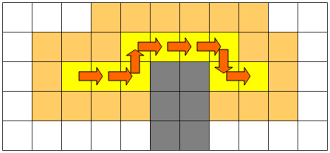
\includegraphics[height=0.2\textwidth]{obstacle.png}\\
%% ~\\
%% \end{center}

%% \begin{itemize}
%% \item Original $A^*$ algorithm~[5]
%% \medskip
%% \item Use of $A^*$ algorithm in route planning~[4] 
%% \end{itemize}
%% \end{frame}

%%%%%%%%%%%%%%%%%%%
%         2       %
%%%%%%%%%%%%%%%%%%%
\begin{frame}
\frametitle{Fast MST by Fredman and Tarjan}

\begin{block}{}
find a spanning tree of an edge-weighted graph with minimum total edge weight 
\end{block}

\begin{itemize}
\item reminder of Prim's algorithm~\cite{krumke09}
%\medskip
\item drawbacks of Prim's algorithm~\cite{krumke09,Eisner97}
%\medskip
\item algorithm by Fredman and Tarjan~\cite{krumke09,Eisner97}
%\medskip
\item running time analysis~\cite{krumke09}
\end{itemize}

\begin{center}
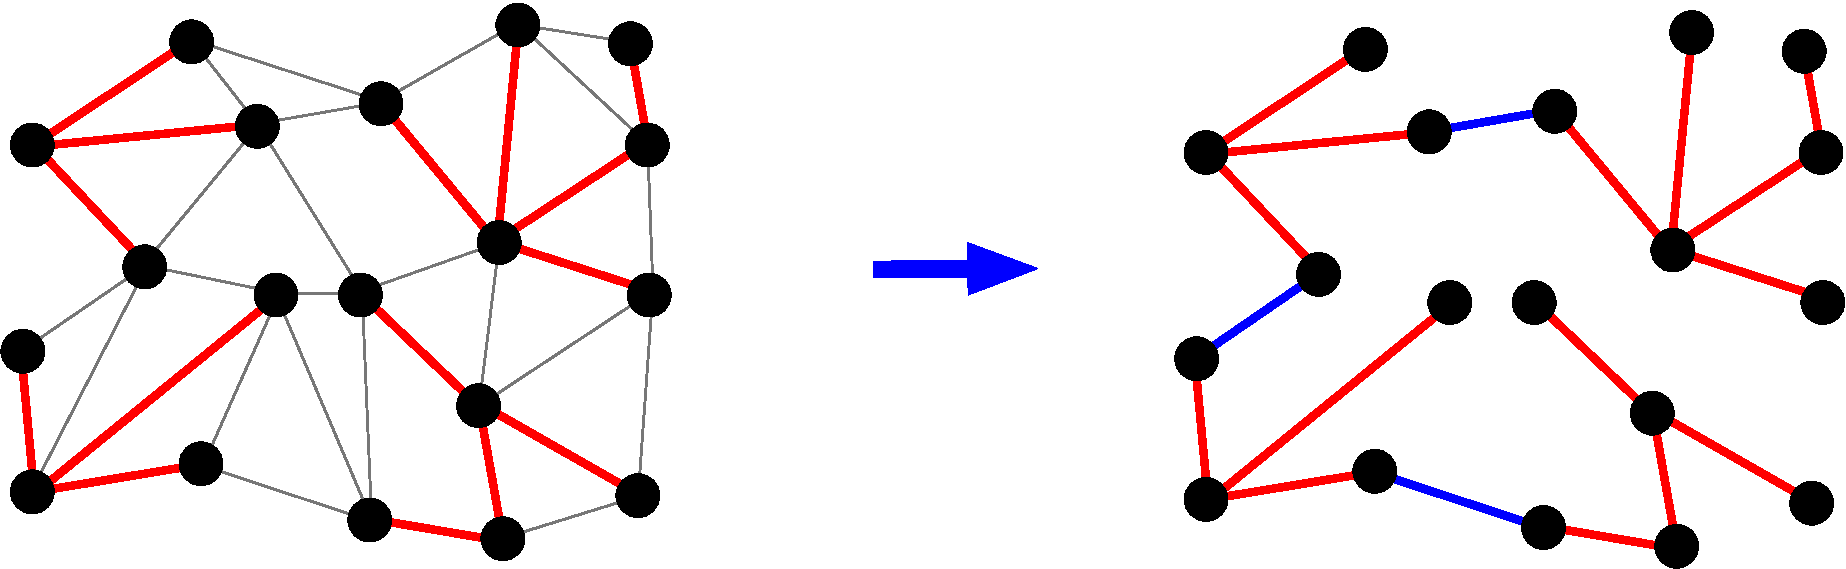
\includegraphics[height=0.2\textwidth]{FredmanTarjan}\\
~\\
From trees to trees of trees (forest)
\end{center}

\end{frame}

%%%%%%%%%%%%%%%%%%%
%         3       %
%%%%%%%%%%%%%%%%%%%
\begin{frame}
  \frametitle{Approximation of Min-Steiner-Trees}
\begin{block}{}
find a tree of minimum edge weight that contains a certain vertex subset (terminals). It may include additional vertices. 
\end{block}


\begin{center}
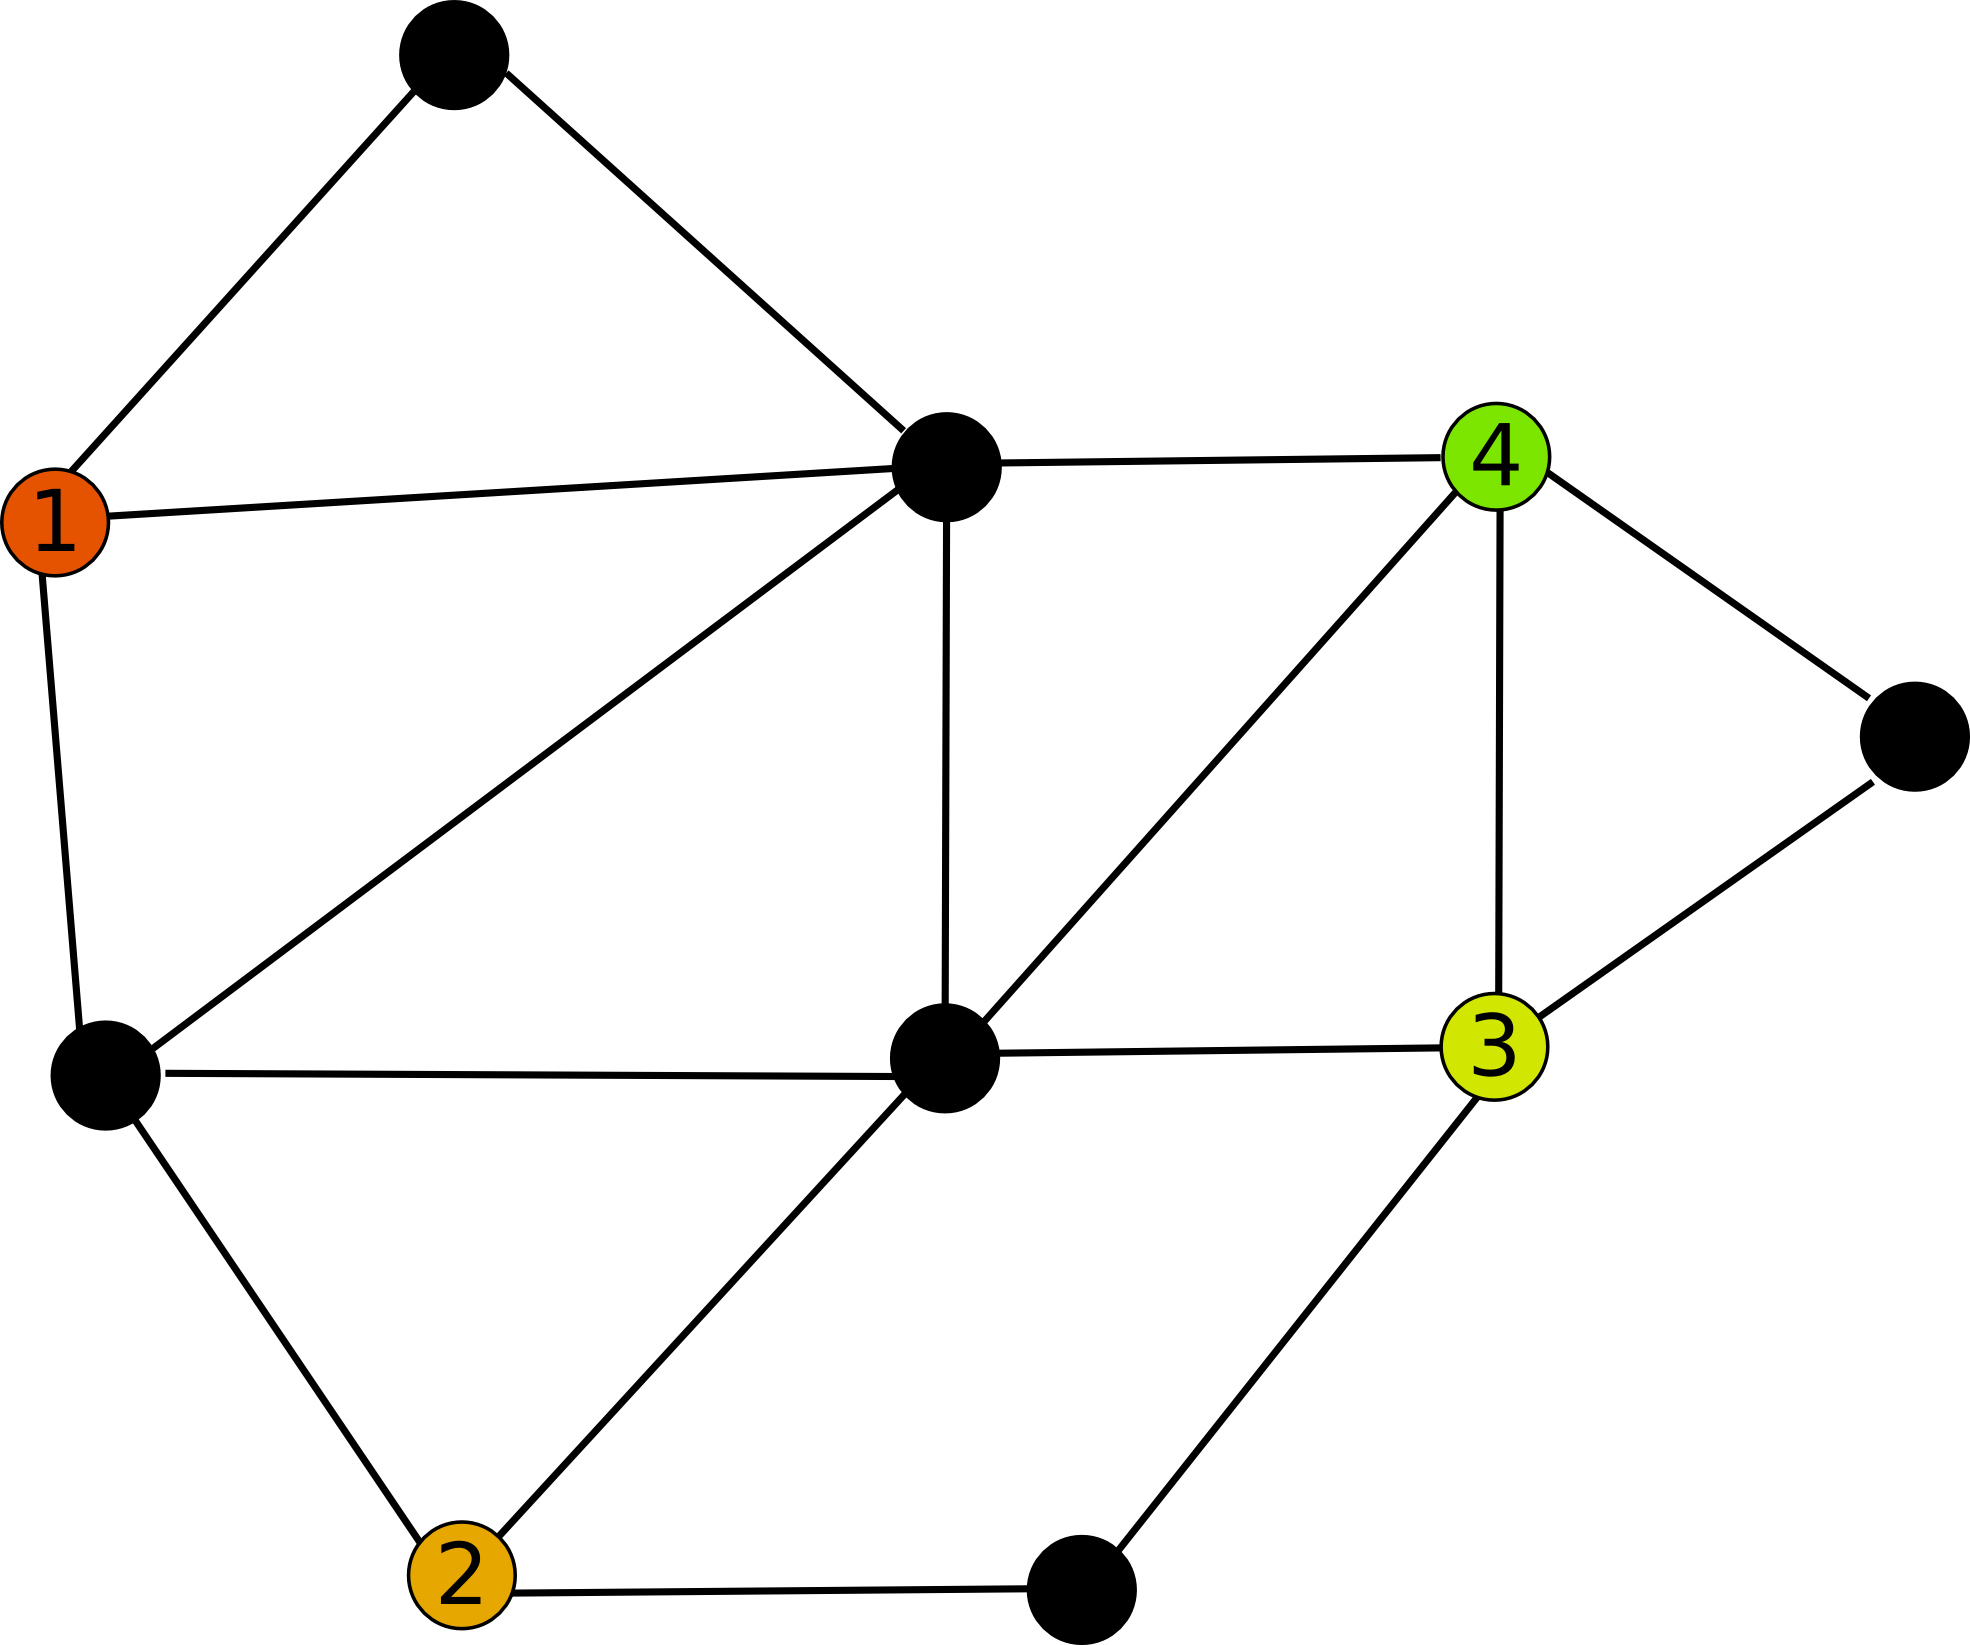
\includegraphics[height=0.22\textwidth]{stree-1.png}\qquad
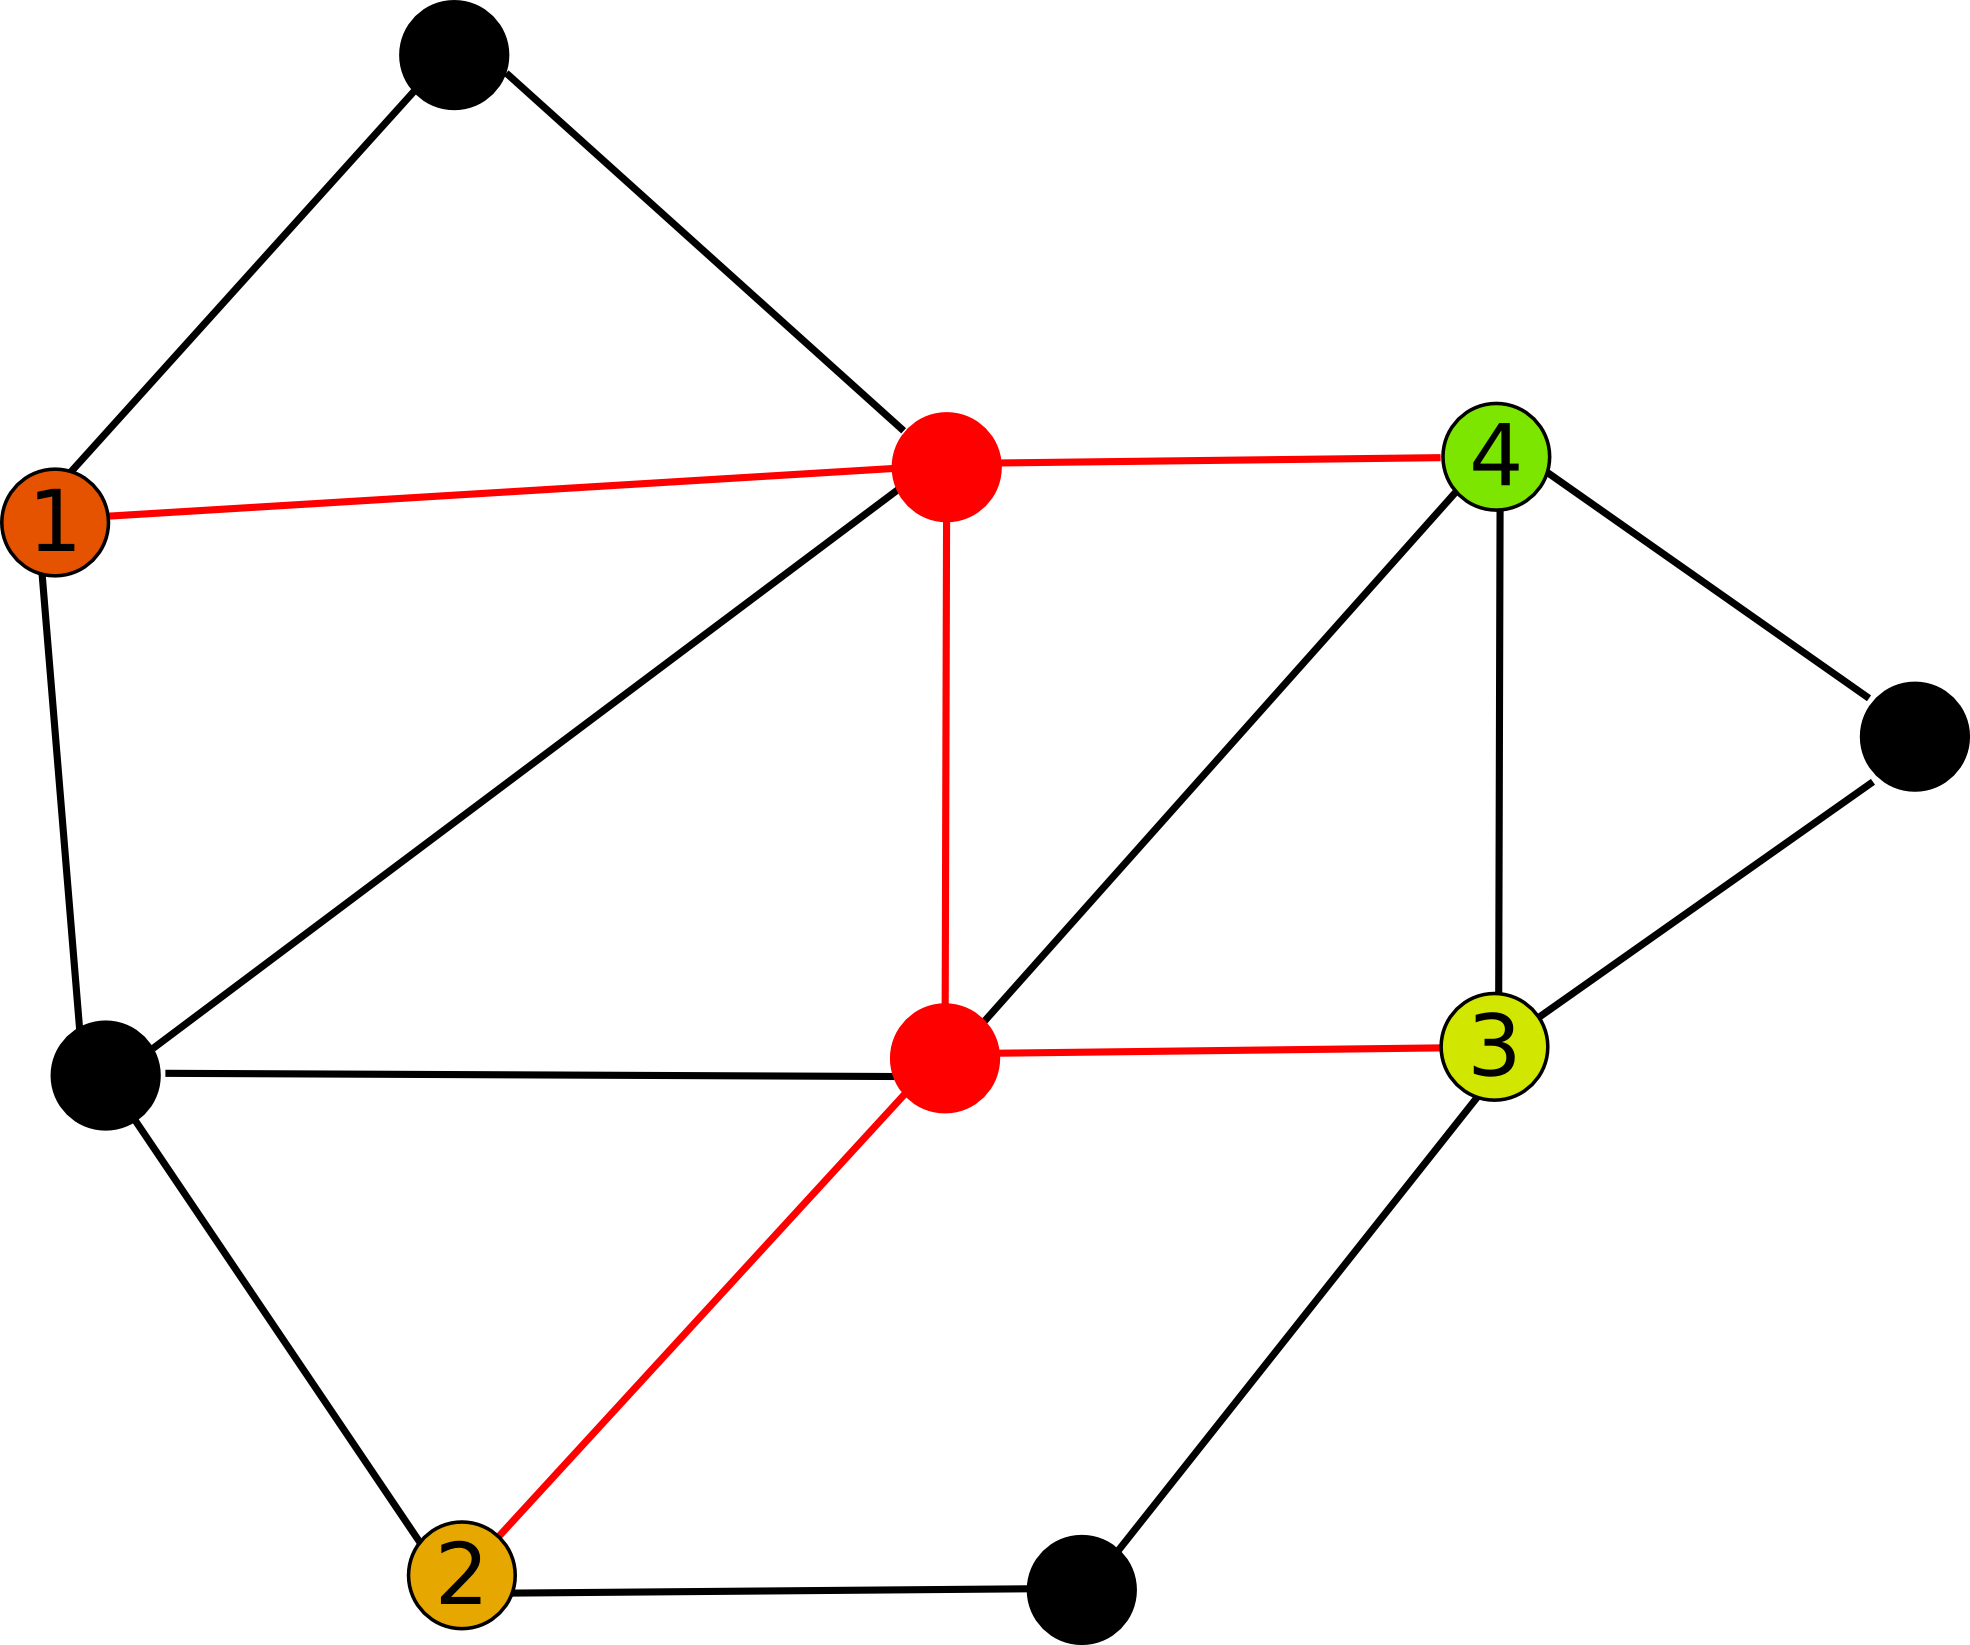
\includegraphics[height=0.22\textwidth]{stree-2.png}\qquad
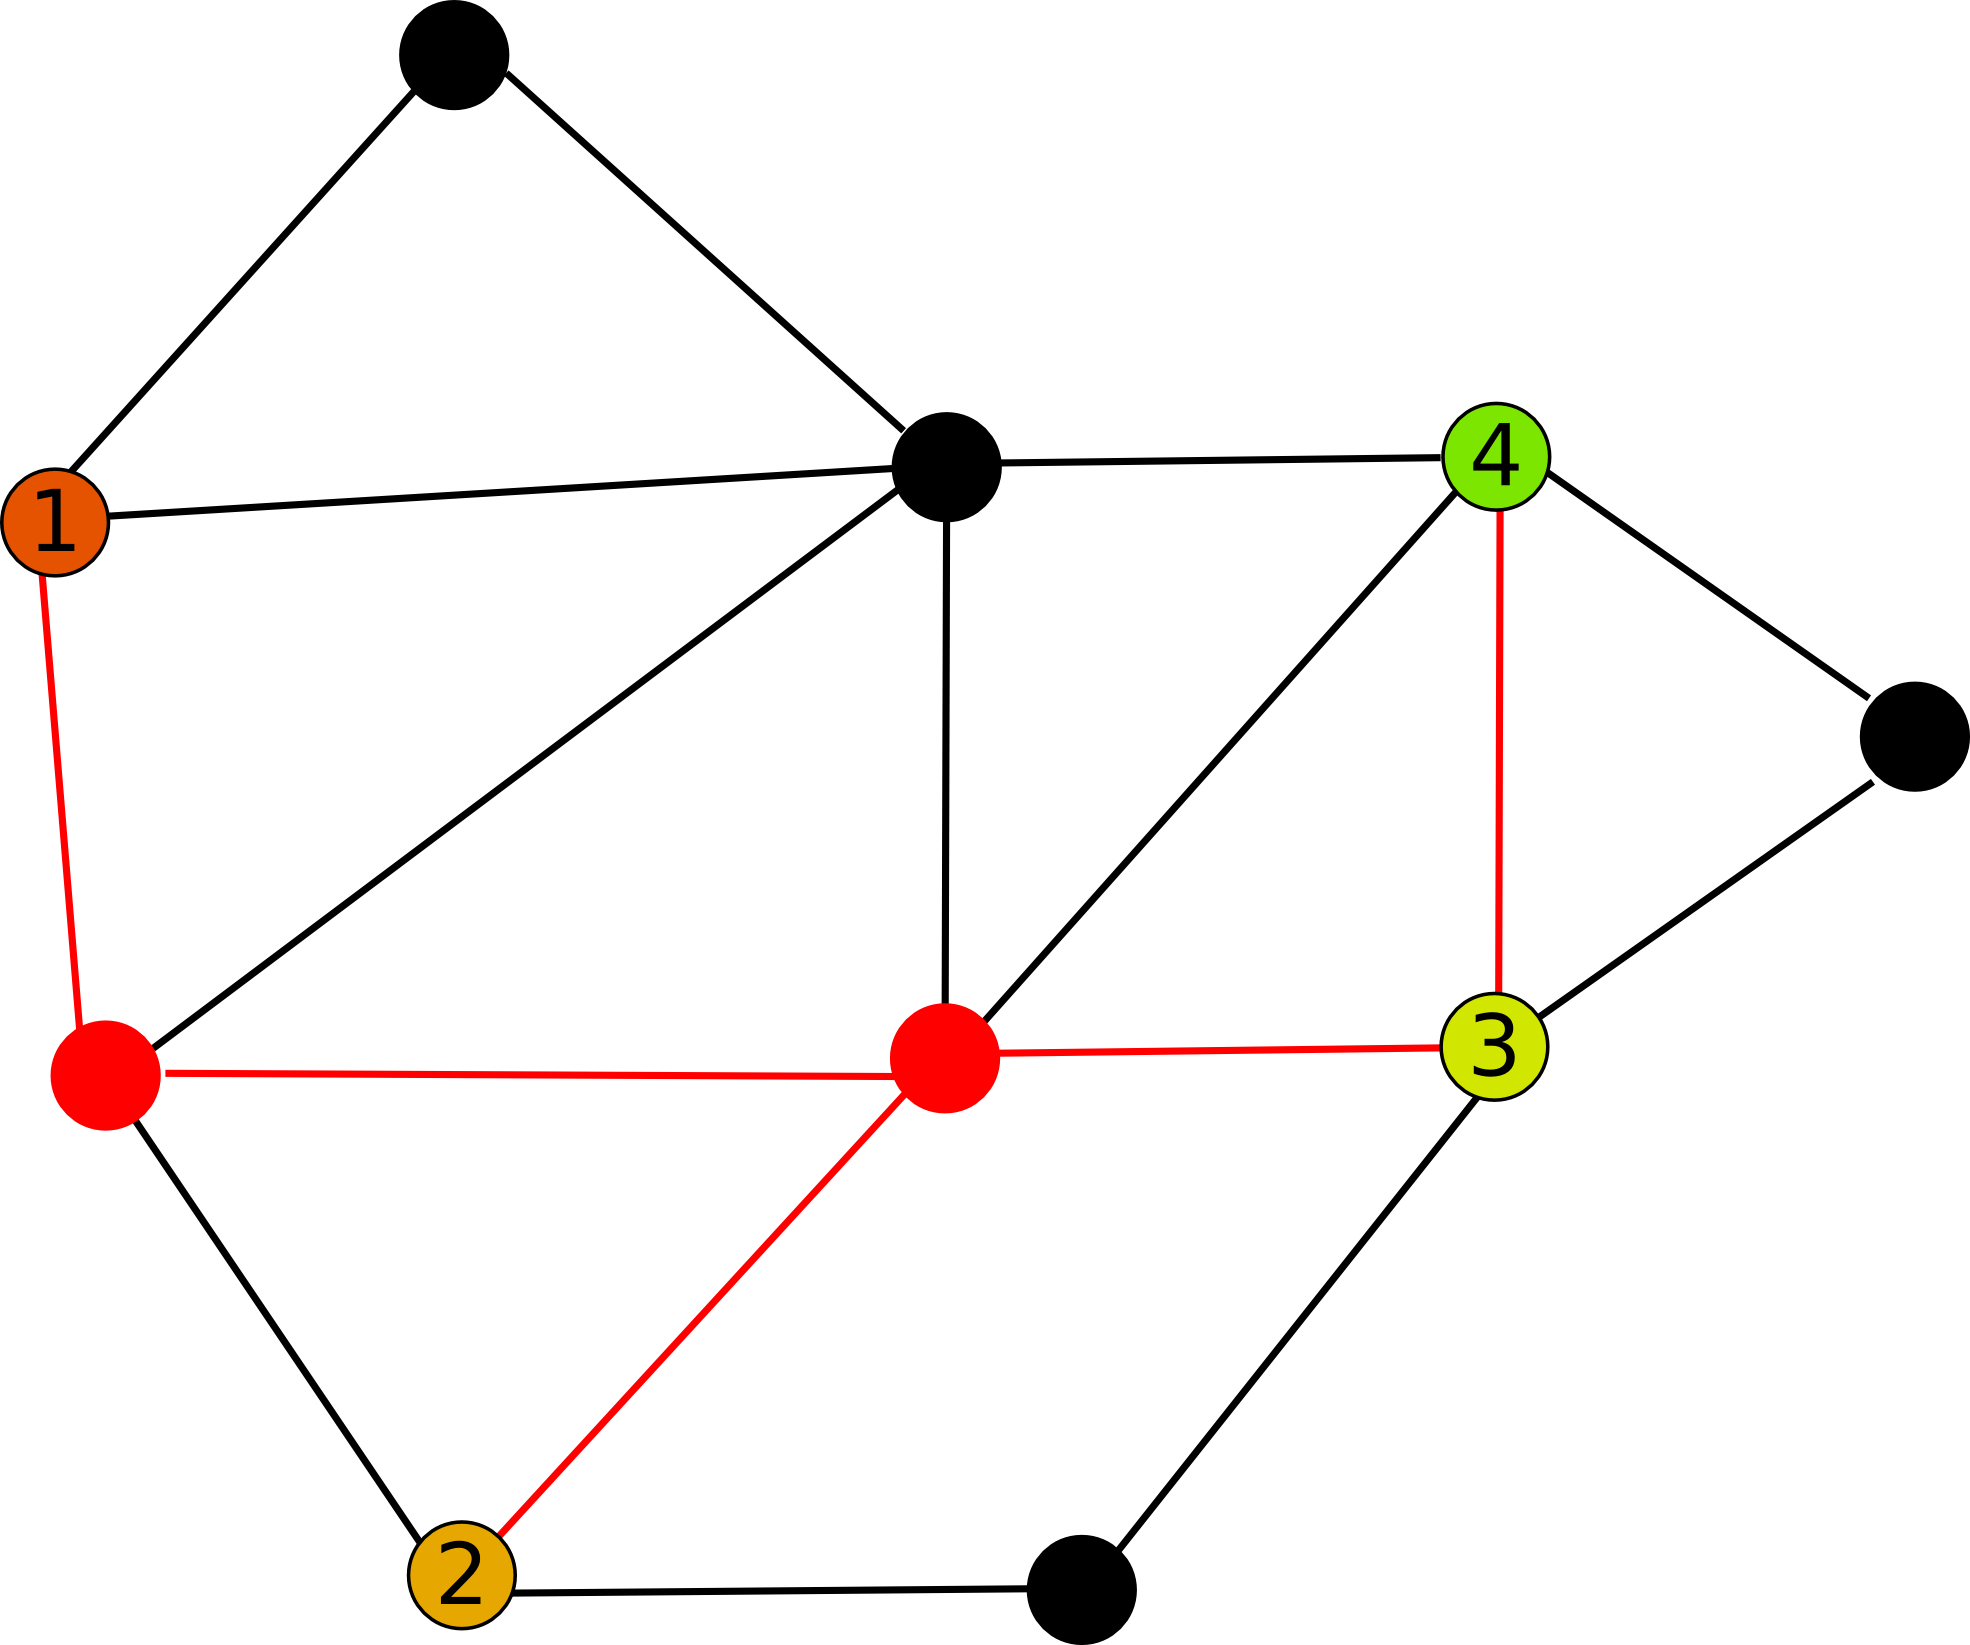
\includegraphics[height=0.22\textwidth]{stree-3.png}

%\includegraphics[height=0.25\textwidth]{figures/steiner1}\qquad
%\includegraphics[height=0.25\textwidth]{figures/steiner2}\qquad
%\includegraphics[height=0.25\textwidth]{figures/steiner3}
\end{center}
~~~~~~$K = \{1, 2, 3, 4\}$~~~~~~~~~~~min Steiner tree~~~~~~~~~~~~~min Steiner tree\\
~\\
\begin{itemize}
\item definitions (terminals, Steiner points)~\cite{krumke09}
%\medskip
\item approximation algorithm for Steiner trees~\cite{krumke09}
\item correctness of algorithm~\cite{krumke09} % solution approximation
\end{itemize}

\end{frame}
  
  
%%%%%%%%%%%%%%%%%%%
%         4       %
%%%%%%%%%%%%%%%%%%%
\begin{frame}
\frametitle{Edge Coloring Problem}

\begin{block}{}
  color the edges of a graph such that no adjacent edges have the same color using
  the fewest possible colors
  \end{block}
\begin{center}
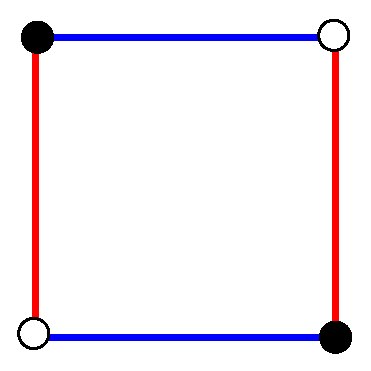
\includegraphics[height=0.25\textwidth]{square}\quad
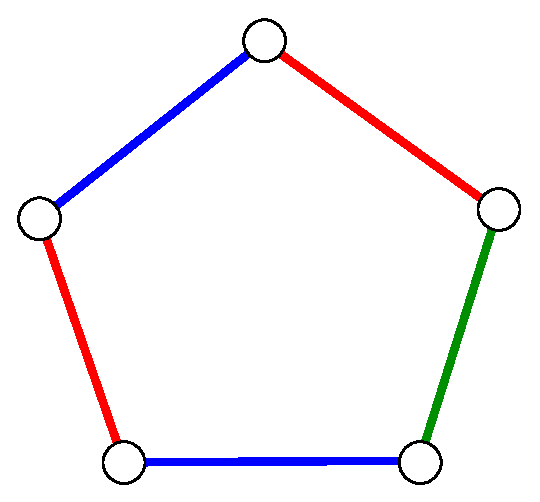
\includegraphics[height=0.25\textwidth]{pentagon}\quad
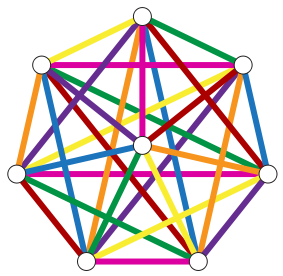
\includegraphics[height=0.3\textwidth]{K7.png}

\end{center}


\begin{itemize}
\item theorems by K\"{o}nig and Vizing on edge chromatic number~\cite{daglib12}
%\item $\chi'(G) = \Delta(G)$ for bipartite graphs~[1]
  %\item $\chi'(G) \leq \Delta(G) + 1$ in general~[1]
  \item chromatic index for bipartite and general graphs~\cite{daglib12}
  \item algorithm by Misra and Gries for general graphs~\cite{Misra92}
  %  \item correctness of algorithm
\end{itemize}

\end{frame}

%%%%%%%%%%%%%%%%%%%
%         5     %
%%%%%%%%%%%%%%%%%%%
% The PageRank algorithm outputs a probability distribution used to represent the likelihood that a person randomly clicking on links will arrive at any particular page.
\begin{frame}
\frametitle{The PageRank Algorithm}
\begin{block}{}
  PageRank algorithm models the structure of pages on the web and measures the importance of each page
\end{block}
\begin{center}
\includegraphics[height=0.25\textwidth]{closeness-exmp.png}\qquad \qquad
\end{center}
\begin{itemize}
\item random surfer model, transition matrix~\cite{Brin98}
\item computation of PageRank vector~\cite{Brin98} % as an eigenvector problem
\item Perron-Frobenius theorem for convergence of Pagerank
\item personilized PageRank~\cite{Jen03}
\end{itemize}

\end{frame}




%% \begin{frame}
%% \frametitle{The Planar Separator Theorem}
%% \begin{center}
%% 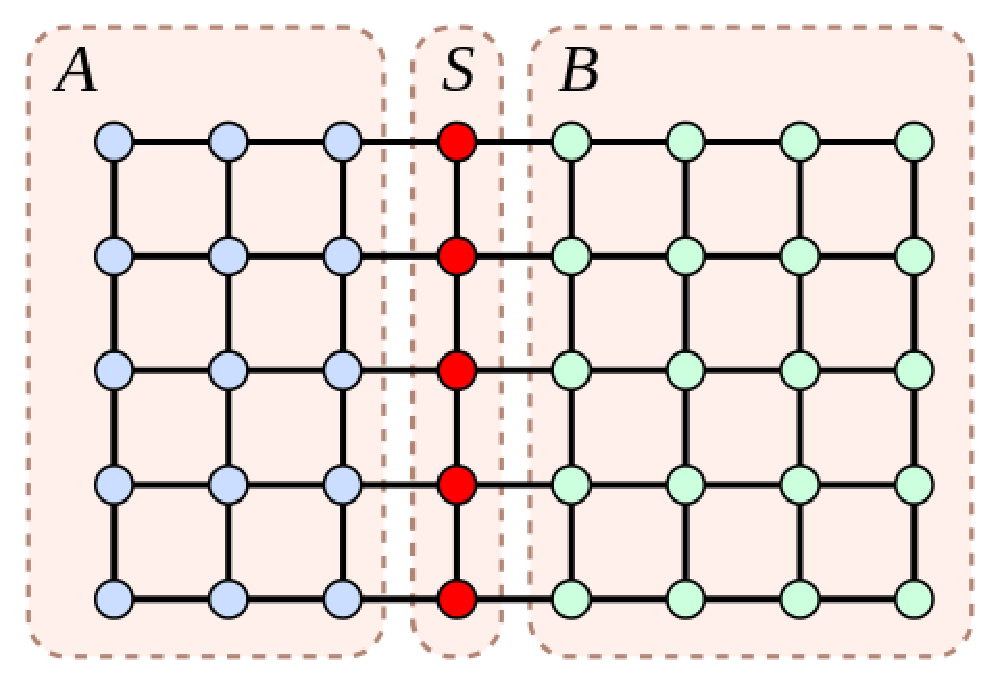
\includegraphics[height=0.3\textwidth]{separator.pdf}\qquad \qquad
%% %\includegraphics[height=0.25\textwidth]{figures/mst}\qquad \qquad
%% %\includegraphics[height=0.2\textwidth]{figures/uniform}
%% \end{center}
%% ~\\
%% \begin{itemize}
%% \item Definition and properties of planar graphs~[1]
%% \medskip
%% \item Kuratowski's Theorem~[1]
%% \medskip
%% \item The algorithm~[11]
%% \end{itemize}
%% \end{frame}


%%%%%%%%%%%%%%%%%%%
%         6       %
%%%%%%%%%%%%%%%%%%%
\begin{frame}
\frametitle{The Assignment Problem}
\begin{block}{}
  find a set of edges without common vertices (matching) in a weighted bipartite graph with maximum weight
\end{block}
\vspace{-1cm}
    \begin{columns}
    \begin{column}{.5\textwidth}
\begin{table}[!ht]
%\small
   \begin{tabular}{|c|c|c|c|} \hline
     workers& Job1 & Job2 & Job3 \\ \hline
     \textcolor{red}{Tom} & \$4  & \$4   & \$4  \\ \hline
     \textcolor{green}{Paul} & \$5 & \$3 & \$6\\  \hline
     \textcolor{yellow}{Helen} &  \$6 & \$3 & \$3 \\ \hline
     \end{tabular}
\end{table} 
\begin{itemize}
\item  relation to max-flow problem, Hungarian algorithm~\cite{daglib12}
\item running time analysis,
\item algorithmic improvements
\end{itemize}
        \end{column}
        \begin{column}{.5\textwidth}
        \centering
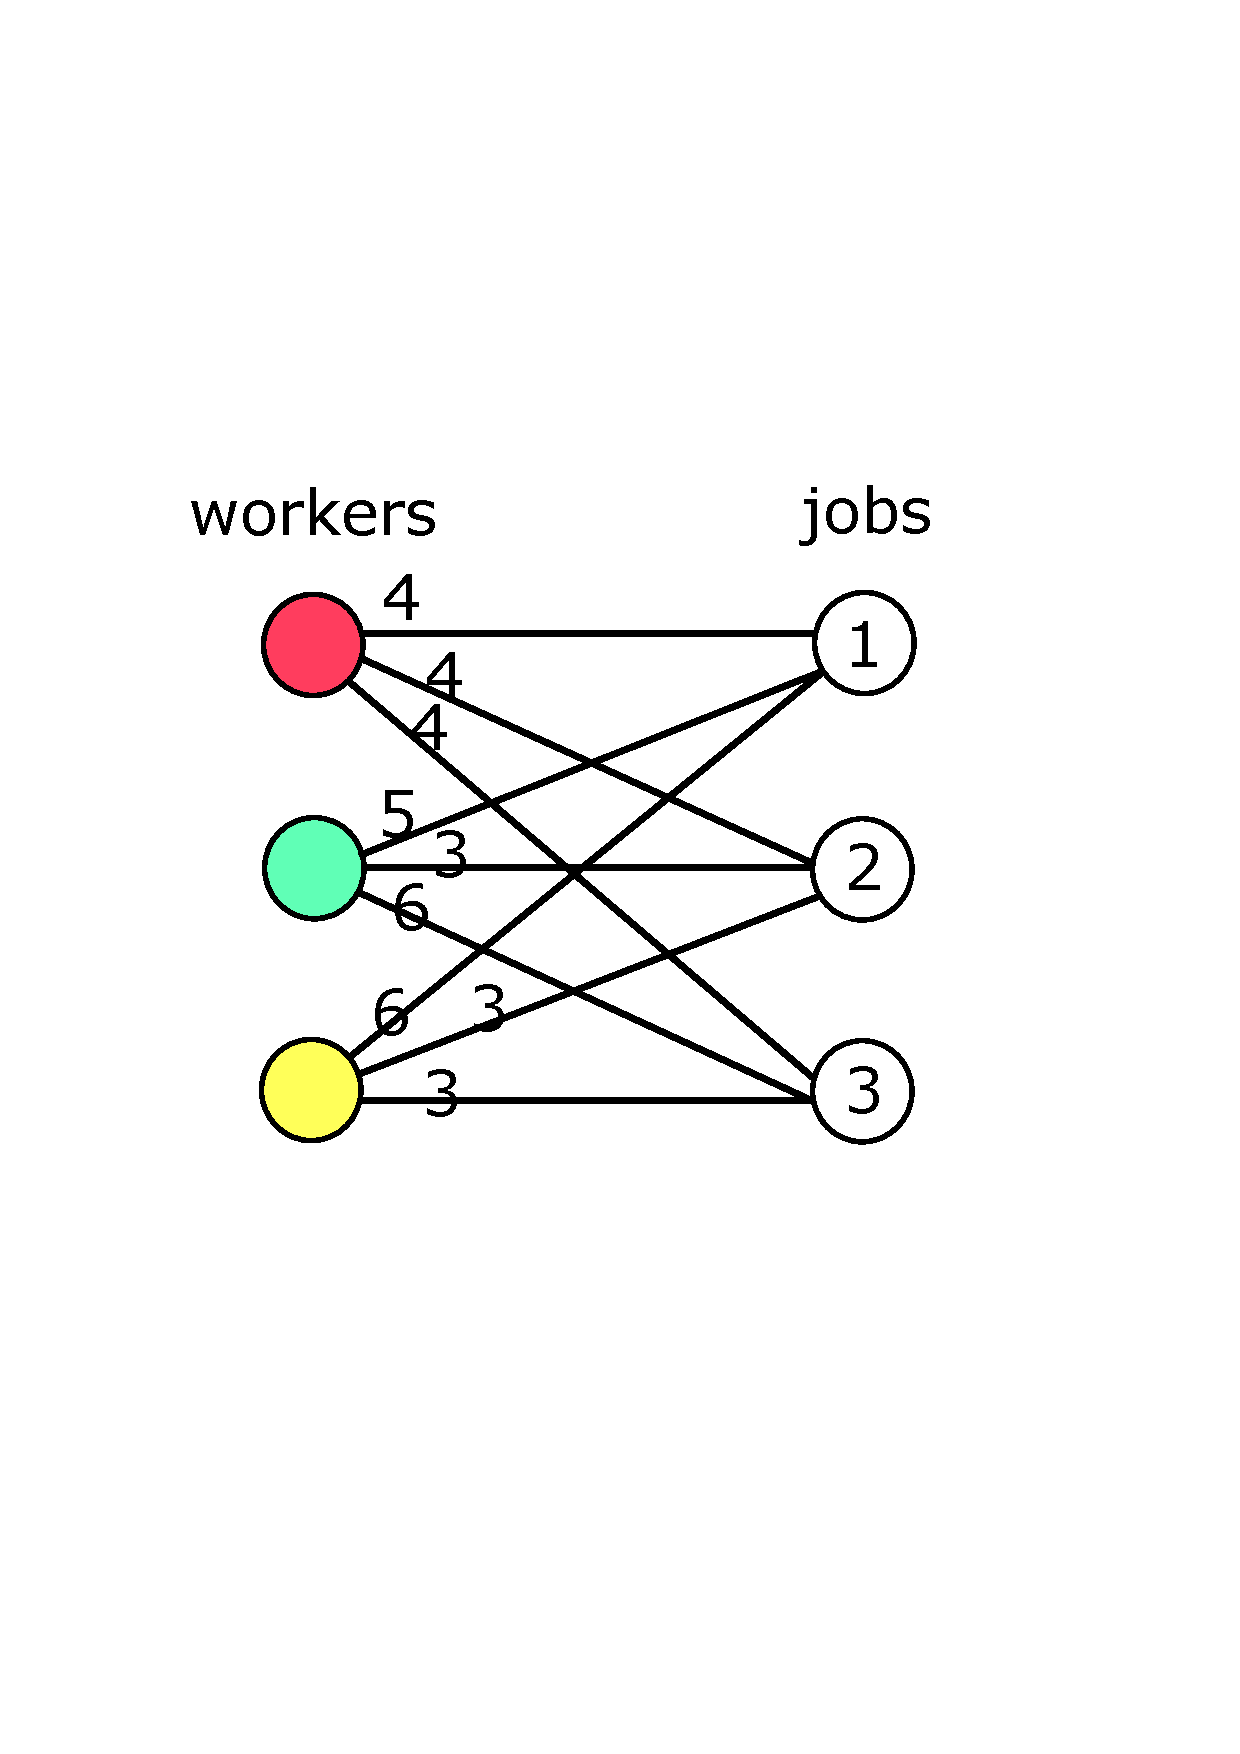
\includegraphics[height=1.3\textwidth]{assignment.pdf}
        \end{column}
        \end{columns}

%\includegraphics[height=0.25\textwidth]{figures/blossom}




\end{frame}
  
%%%%%%%%%%%%%%%%%%%
%         6       %
%%%%%%%%%%%%%%%%%%%
\begin{frame}
\frametitle{ The Blossom Algorithm} %  for Maximum Matching
\begin{block}{}
 find maximum weight matching in a general graph
  \end{block}
\begin{center}
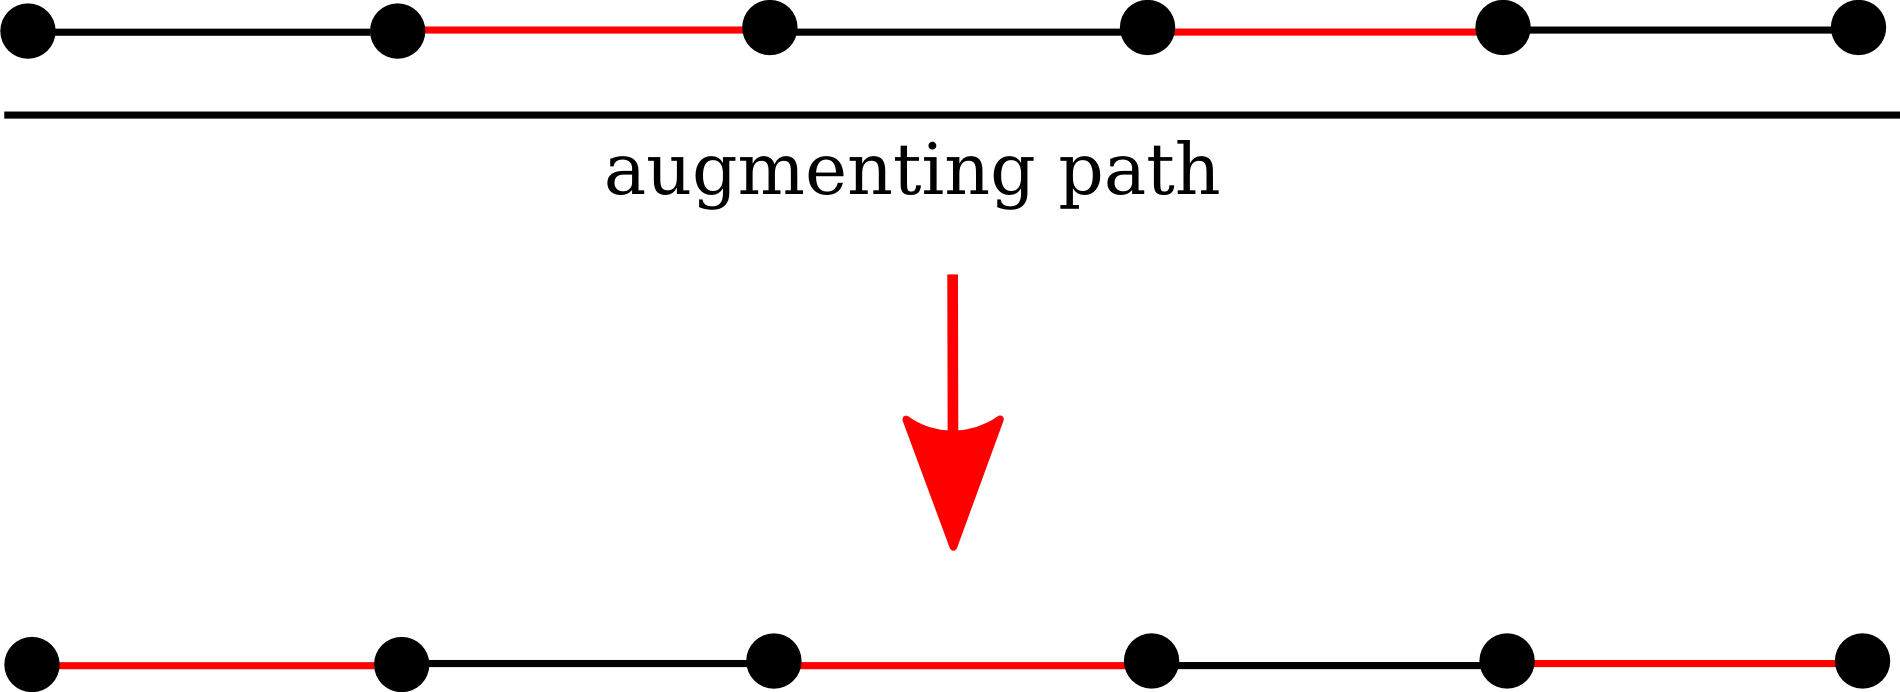
\includegraphics[height=0.25\textwidth]{blossom-matching.png}
%\includegraphics[height=0.25\textwidth]{figures/blossom}
\end{center}

\begin{itemize}
\item finding augmenting paths~\cite{Edmonds65}
\item blossoms and blossom contraction~\cite{Edmonds65}
\item running time analysis
\end{itemize}

\end{frame}

%%%%%%%%%%%%%%%%%%%
%         7       %
%%%%%%%%%%%%%%%%%%%
\begin{frame}
\frametitle{Minimum Cuts by Karger and Stein}
\begin{block}{}
  find a partition of the vertices of a graph with the minimum number of edges whose endpoints are in different parts
\end{block}
  %\begin{center}
%~~~~~~~~graph~~~~~~~~~~~~~~~~~~~~~~~~~~~~\textcolor{blue}{contraction}~~~~~~~~~~~~~~~~~~~~~~~~\textcolor{red}{min cut}~\\
%\centering 
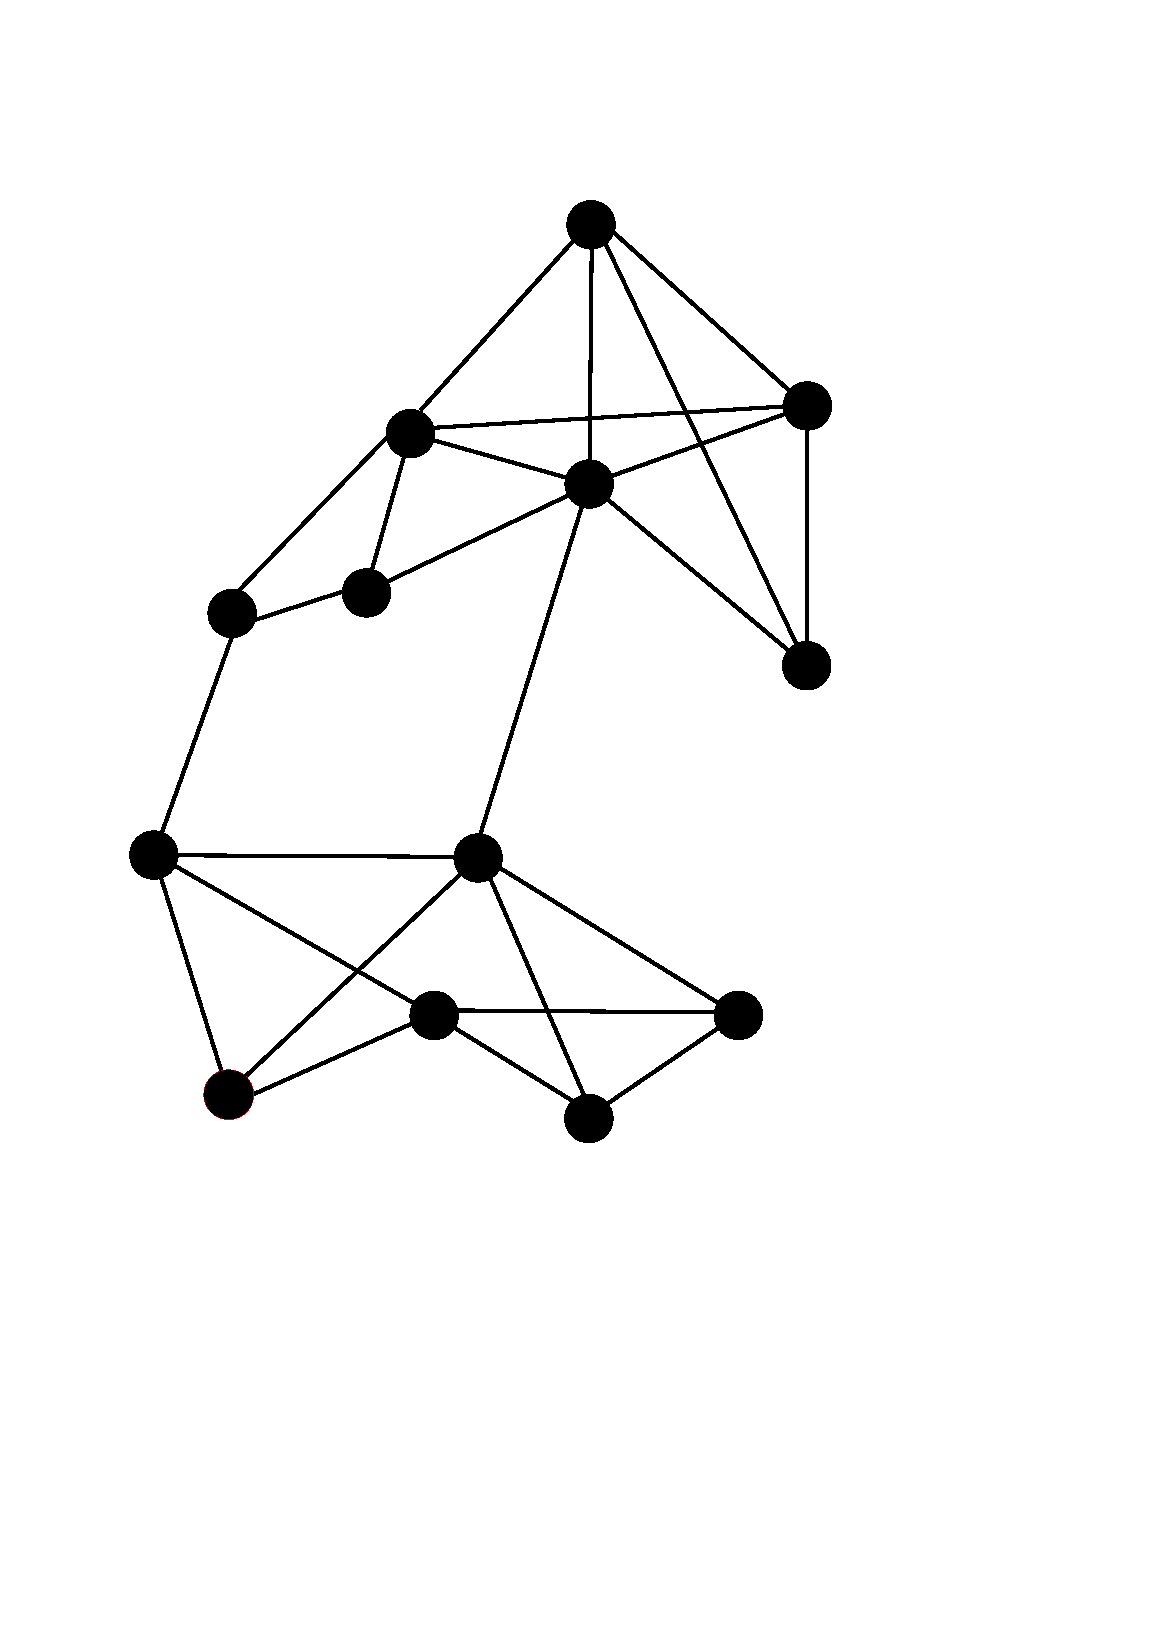
\includegraphics[height=0.6\textheight]{min-cut-1.pdf}
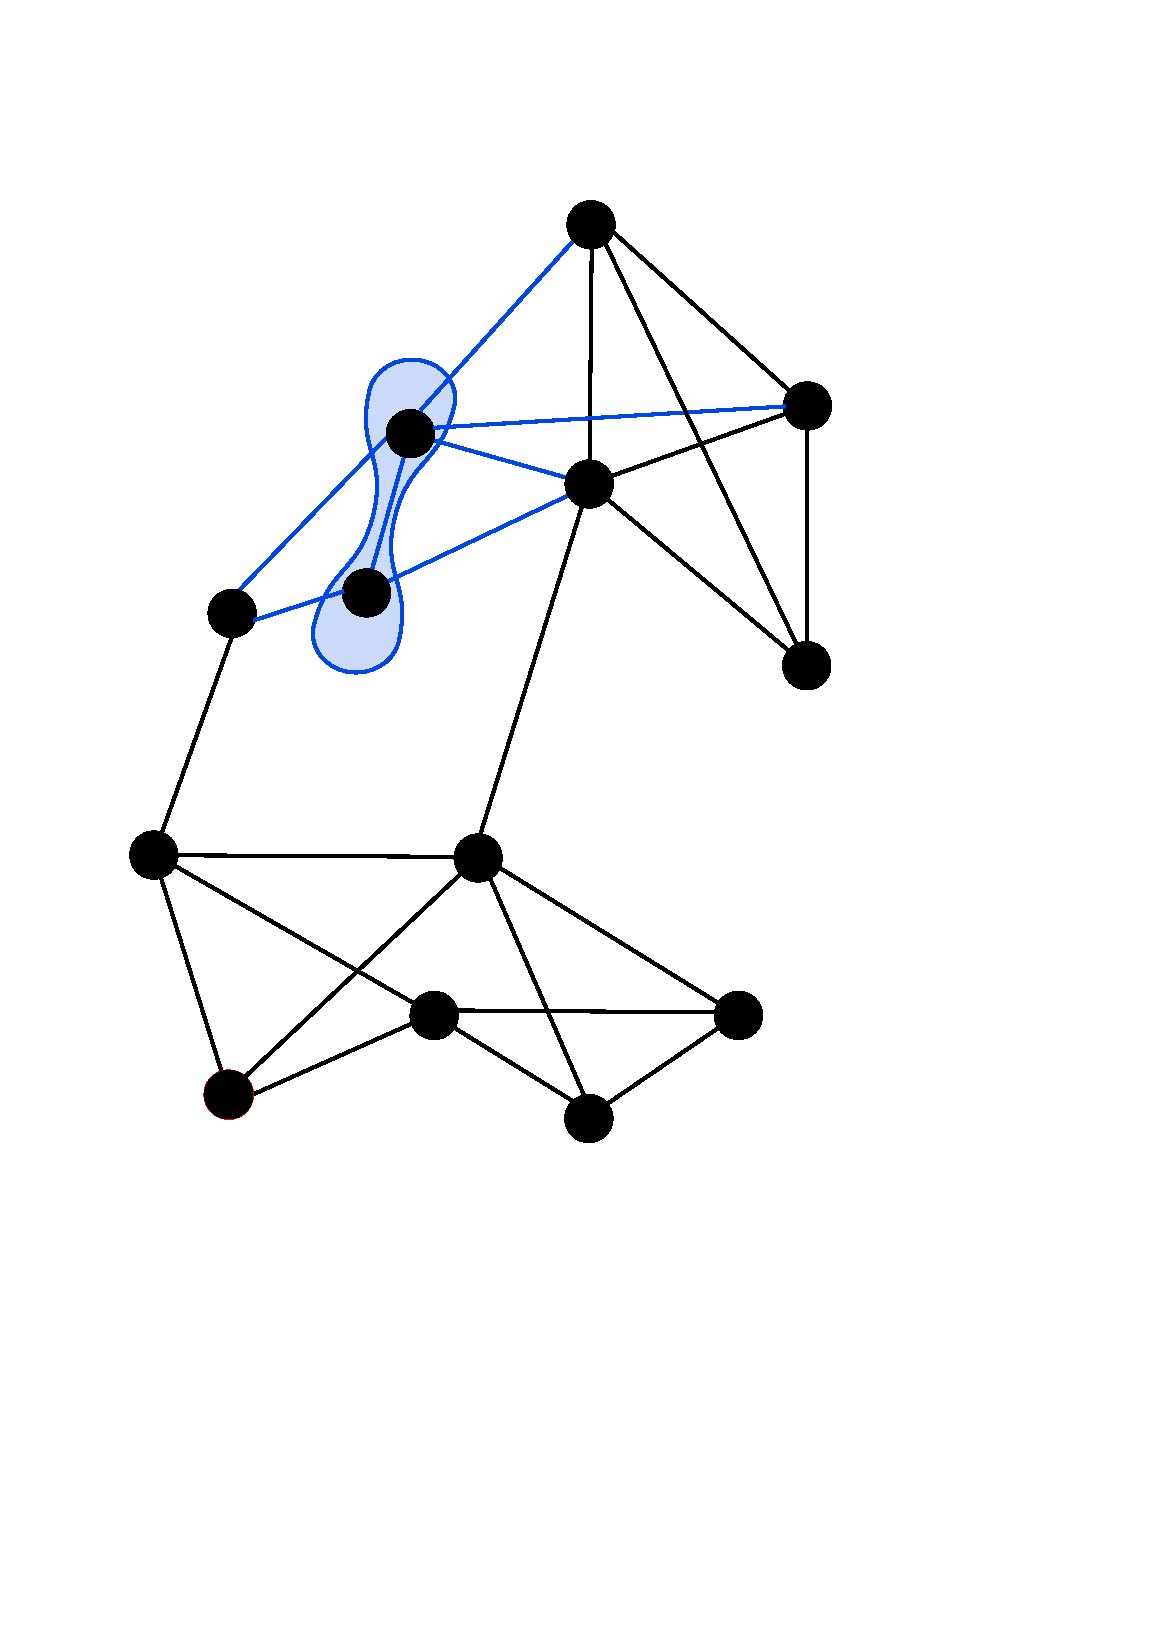
\includegraphics[height=0.6\textheight]{min-cut-3.pdf}
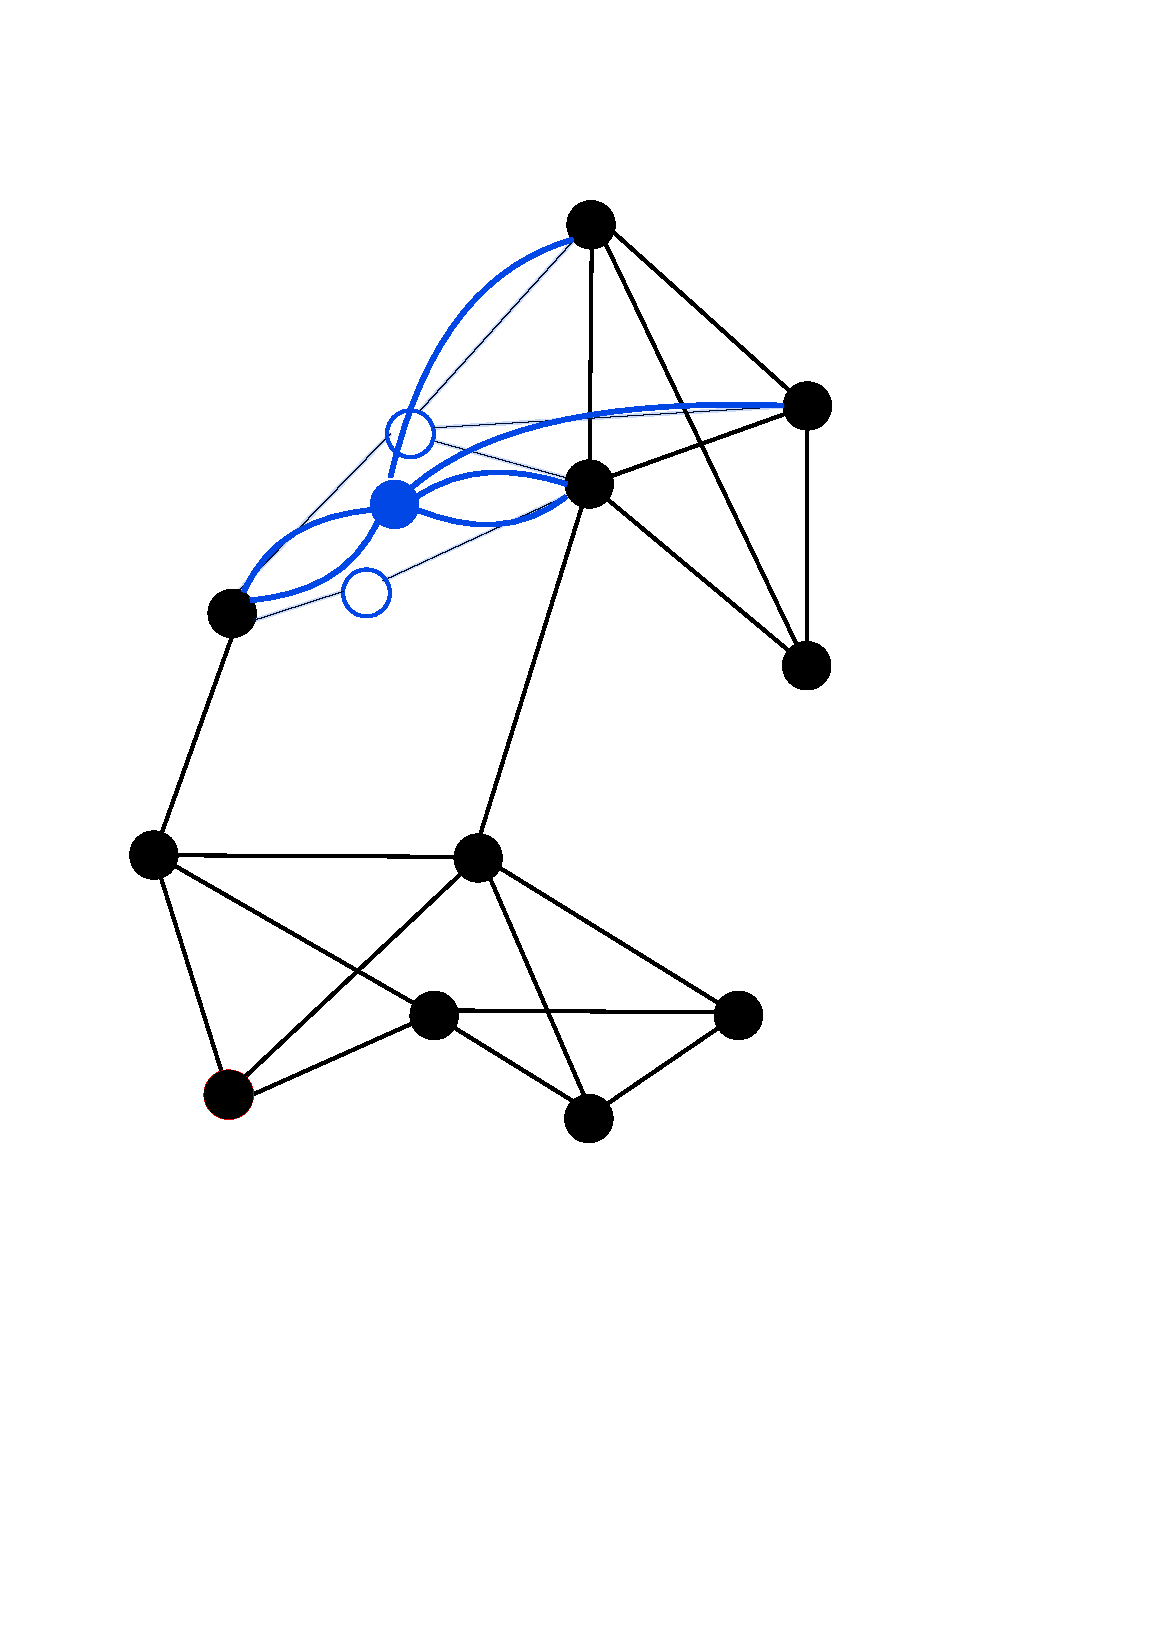
\includegraphics[height=0.6\textheight]{min-cut-5.pdf} 
%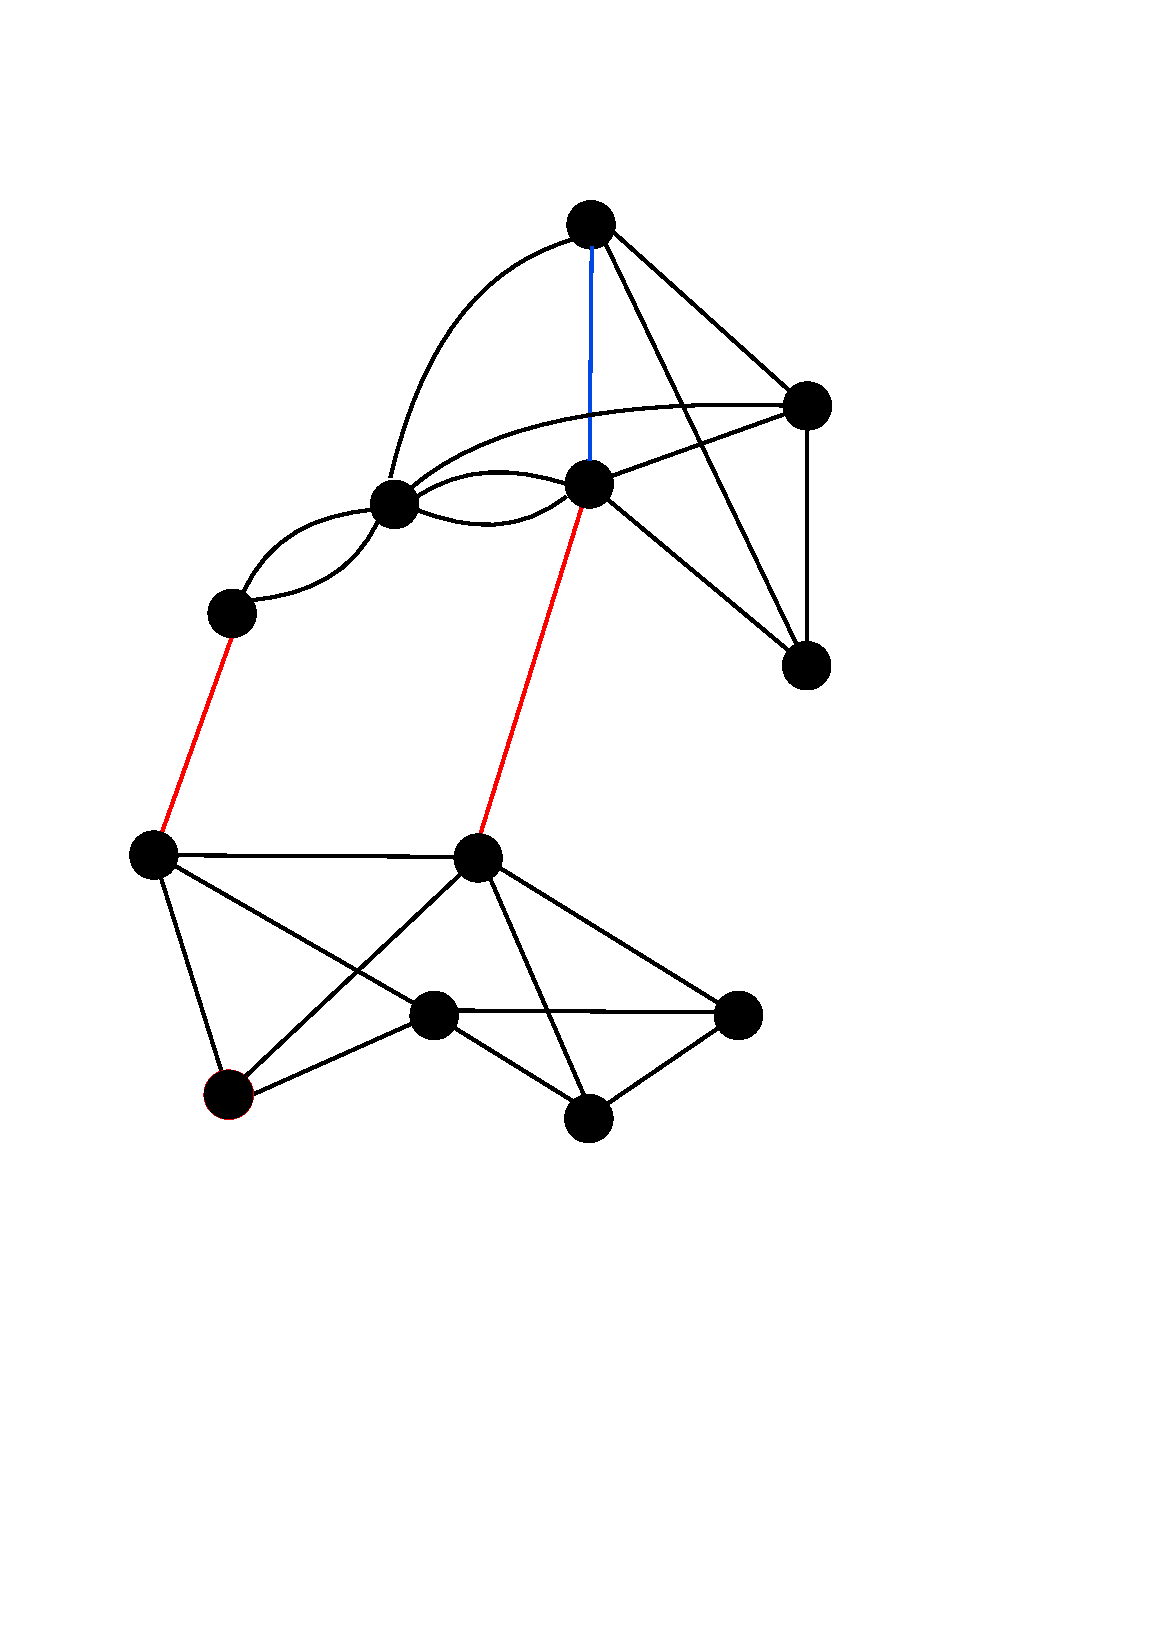
\includegraphics[height=0.5\textheight]{figures/min-cut-6.pdf}
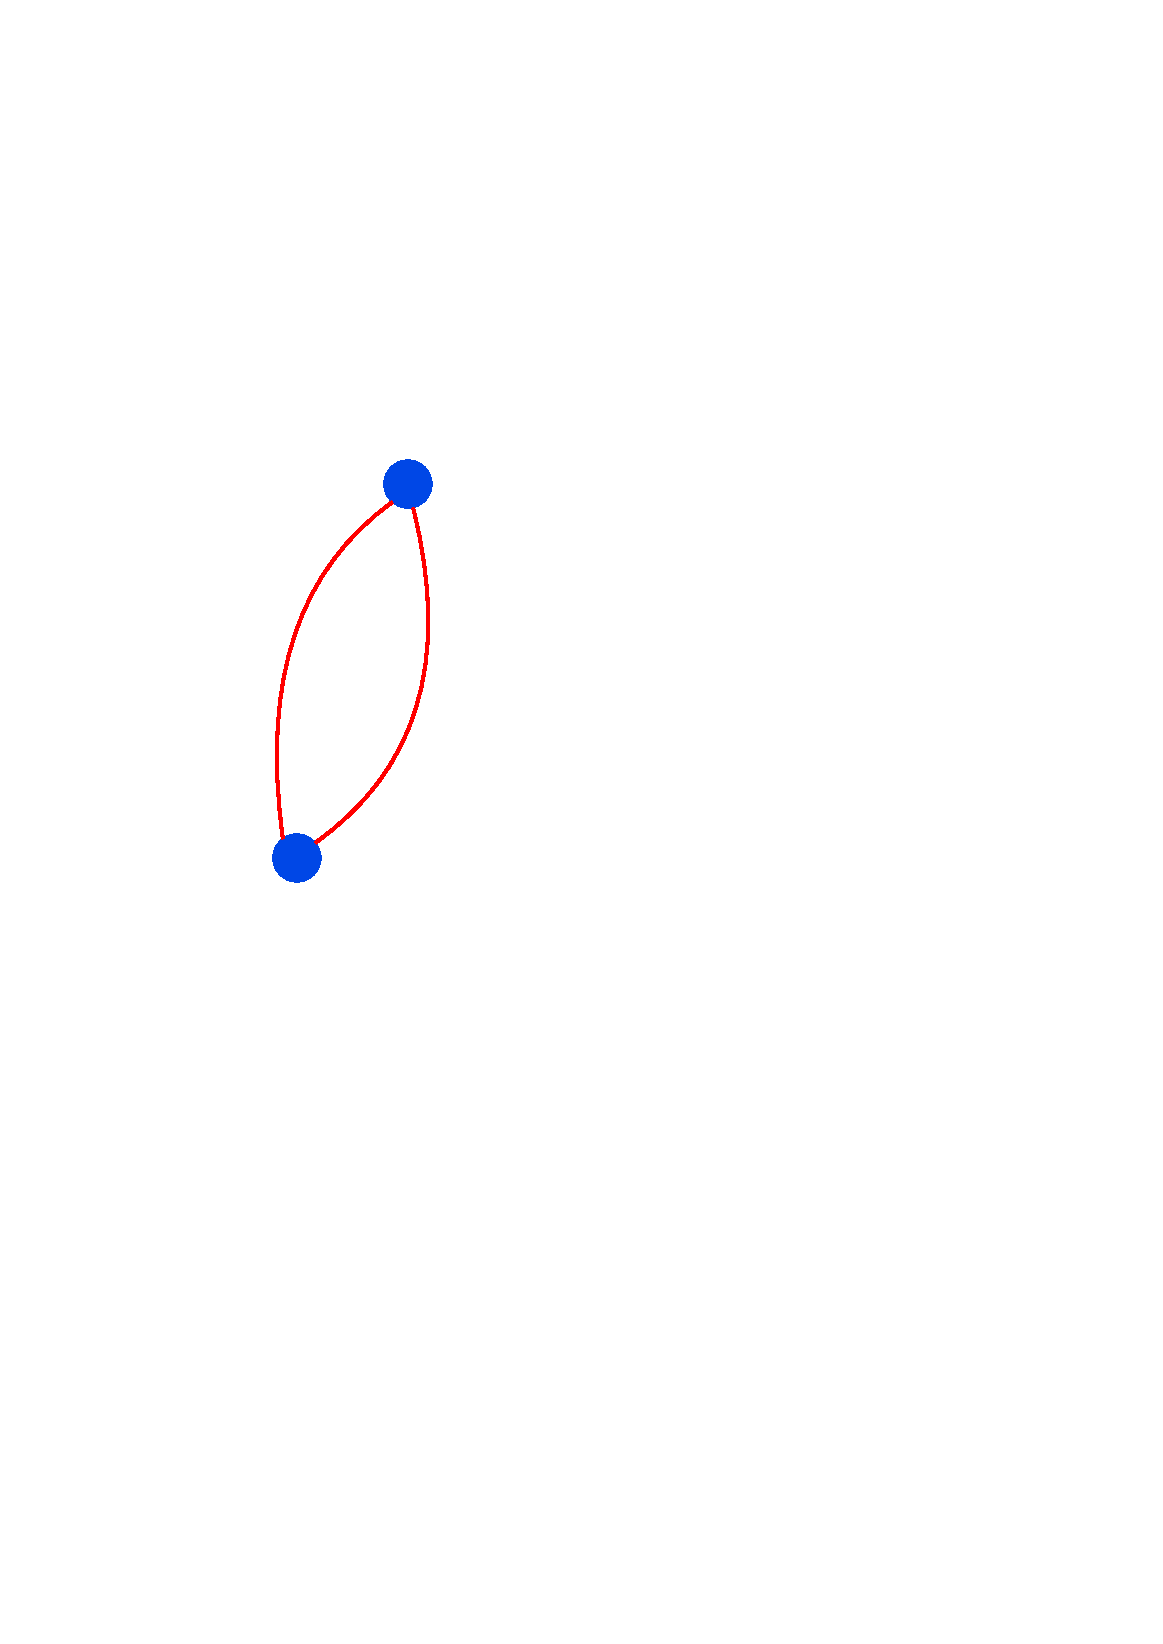
\includegraphics[height=0.6\textheight]{min-cut-7.pdf}
%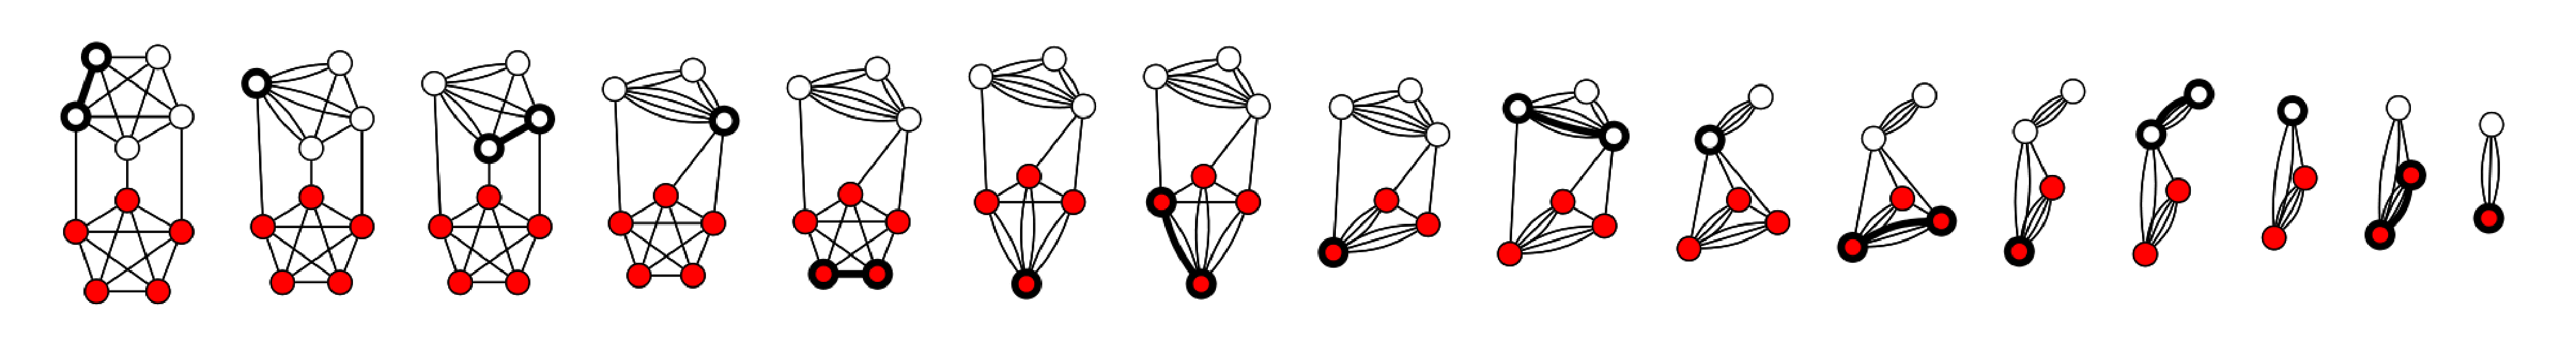
\includegraphics[height=0.25\textwidth]{figures/my_contraction}
%\includegraphics[height=0.25\textwidth]{figures/minCut}\qquad \qquad
%\includegraphics[height=0.25\textwidth]{figures/contraction}
%\end{center}
\vspace{-1cm}
\begin{itemize}
\item edge contraction: definition and implementation~\cite{Karger96}
\item success probability~\cite{Karger96}
\item Karger-Stein algorithm~\cite{Karger96}
\end{itemize}

\end{frame}

%%%%%%%%%%%%%%%%%%%
%         8      %
%%%%%%%%%%%%%%%%%%%
\begin{frame}
  \frametitle{Spectral Partitioning}
  \begin{block}{}
   find a balanced partition of the vertices in a graph such that the number of edges with endpoints in different parts is minimized
    \end{block}
\begin{center}
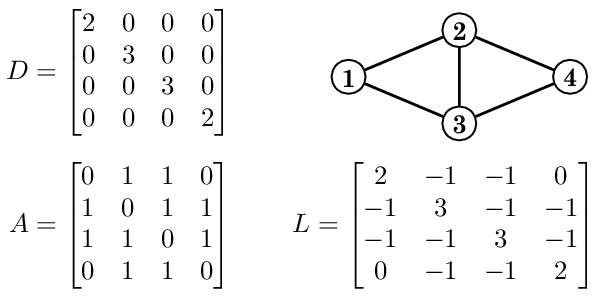
\includegraphics[height=0.3\textwidth]{laplacian-2}\qquad \qquad
%\includegraphics[height=0.25\textwidth]{figures/mst}\qquad \qquad
%\includegraphics[height=0.2\textwidth]{figures/uniform}
\end{center}
~\\
\begin{itemize}
\item Laplacian and properties~\cite{Bichot2013} % laplacian eigenvalues
\item Fiedler eigenvalue and eigenvector~\cite{Fiedler73}
\end{itemize}

\end{frame}


%%%%%%%%%%%%%%%%%%%
%         9       %
%%%%%%%%%%%%%%%%%%%
\begin{frame}
\frametitle{Tree Decomposition}
\begin{block}{}
  find a decomposition of the graph that represents the vertices of a given graph G as subtrees of a tree
\end{block}
\begin{center}
%\includegraphics[height=0.25\textwidth]{figures/treeDecomp}
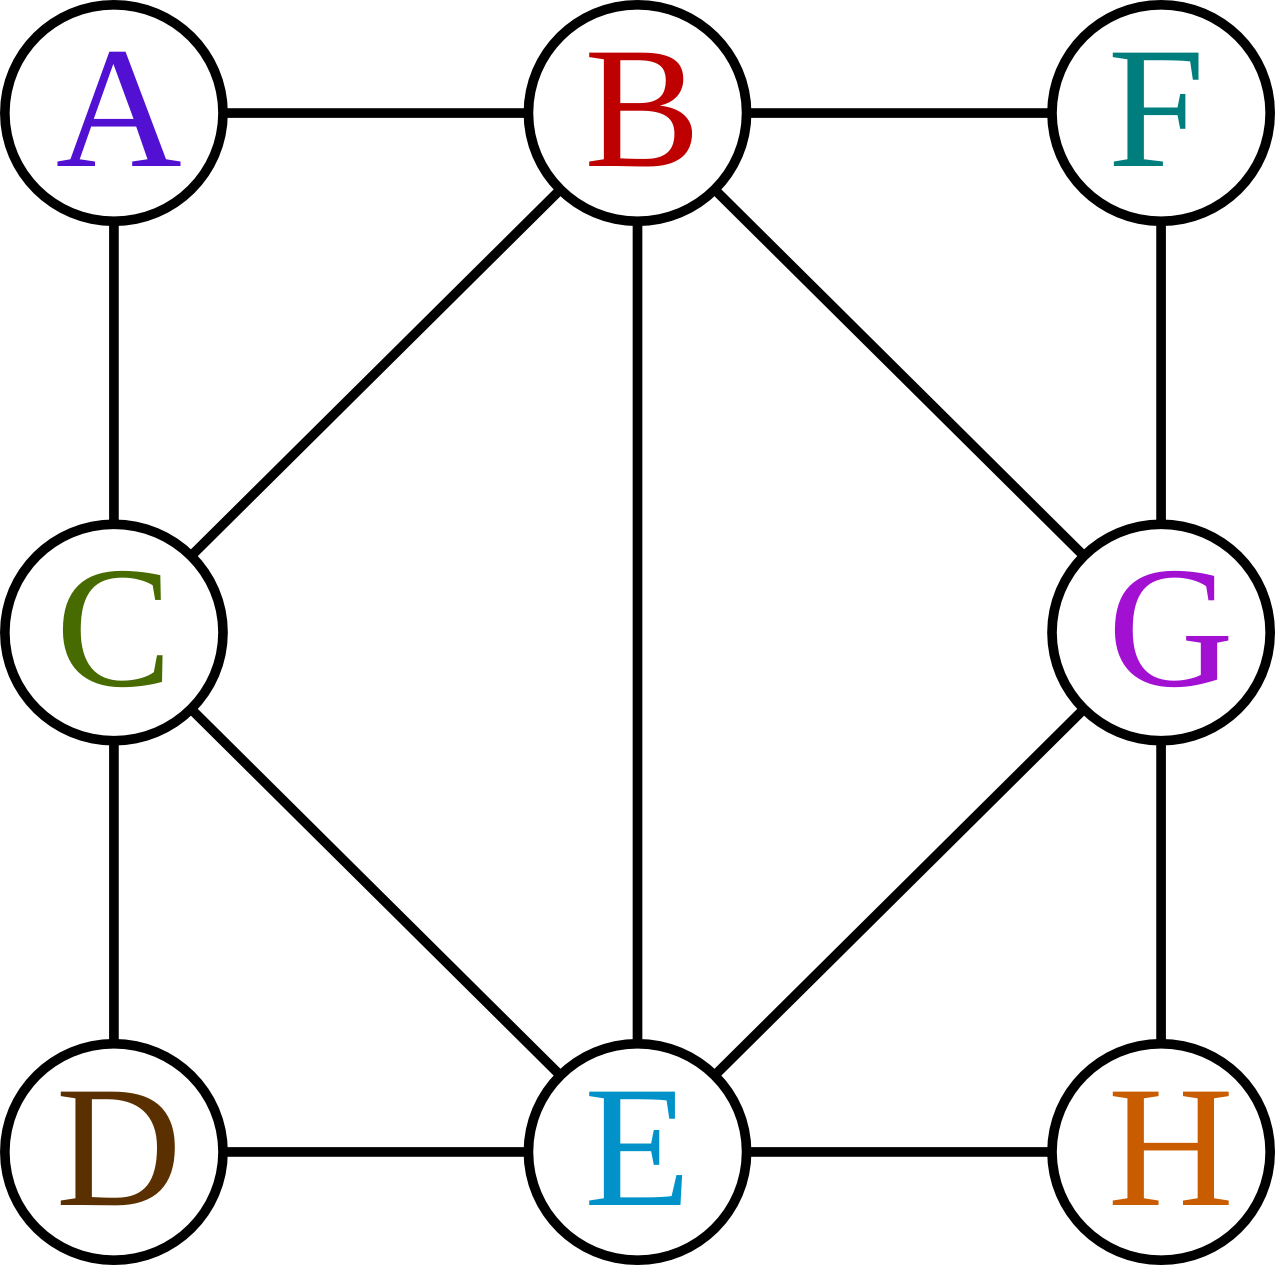
\includegraphics[height=0.37\textheight]{my_tree_3.png}\qquad
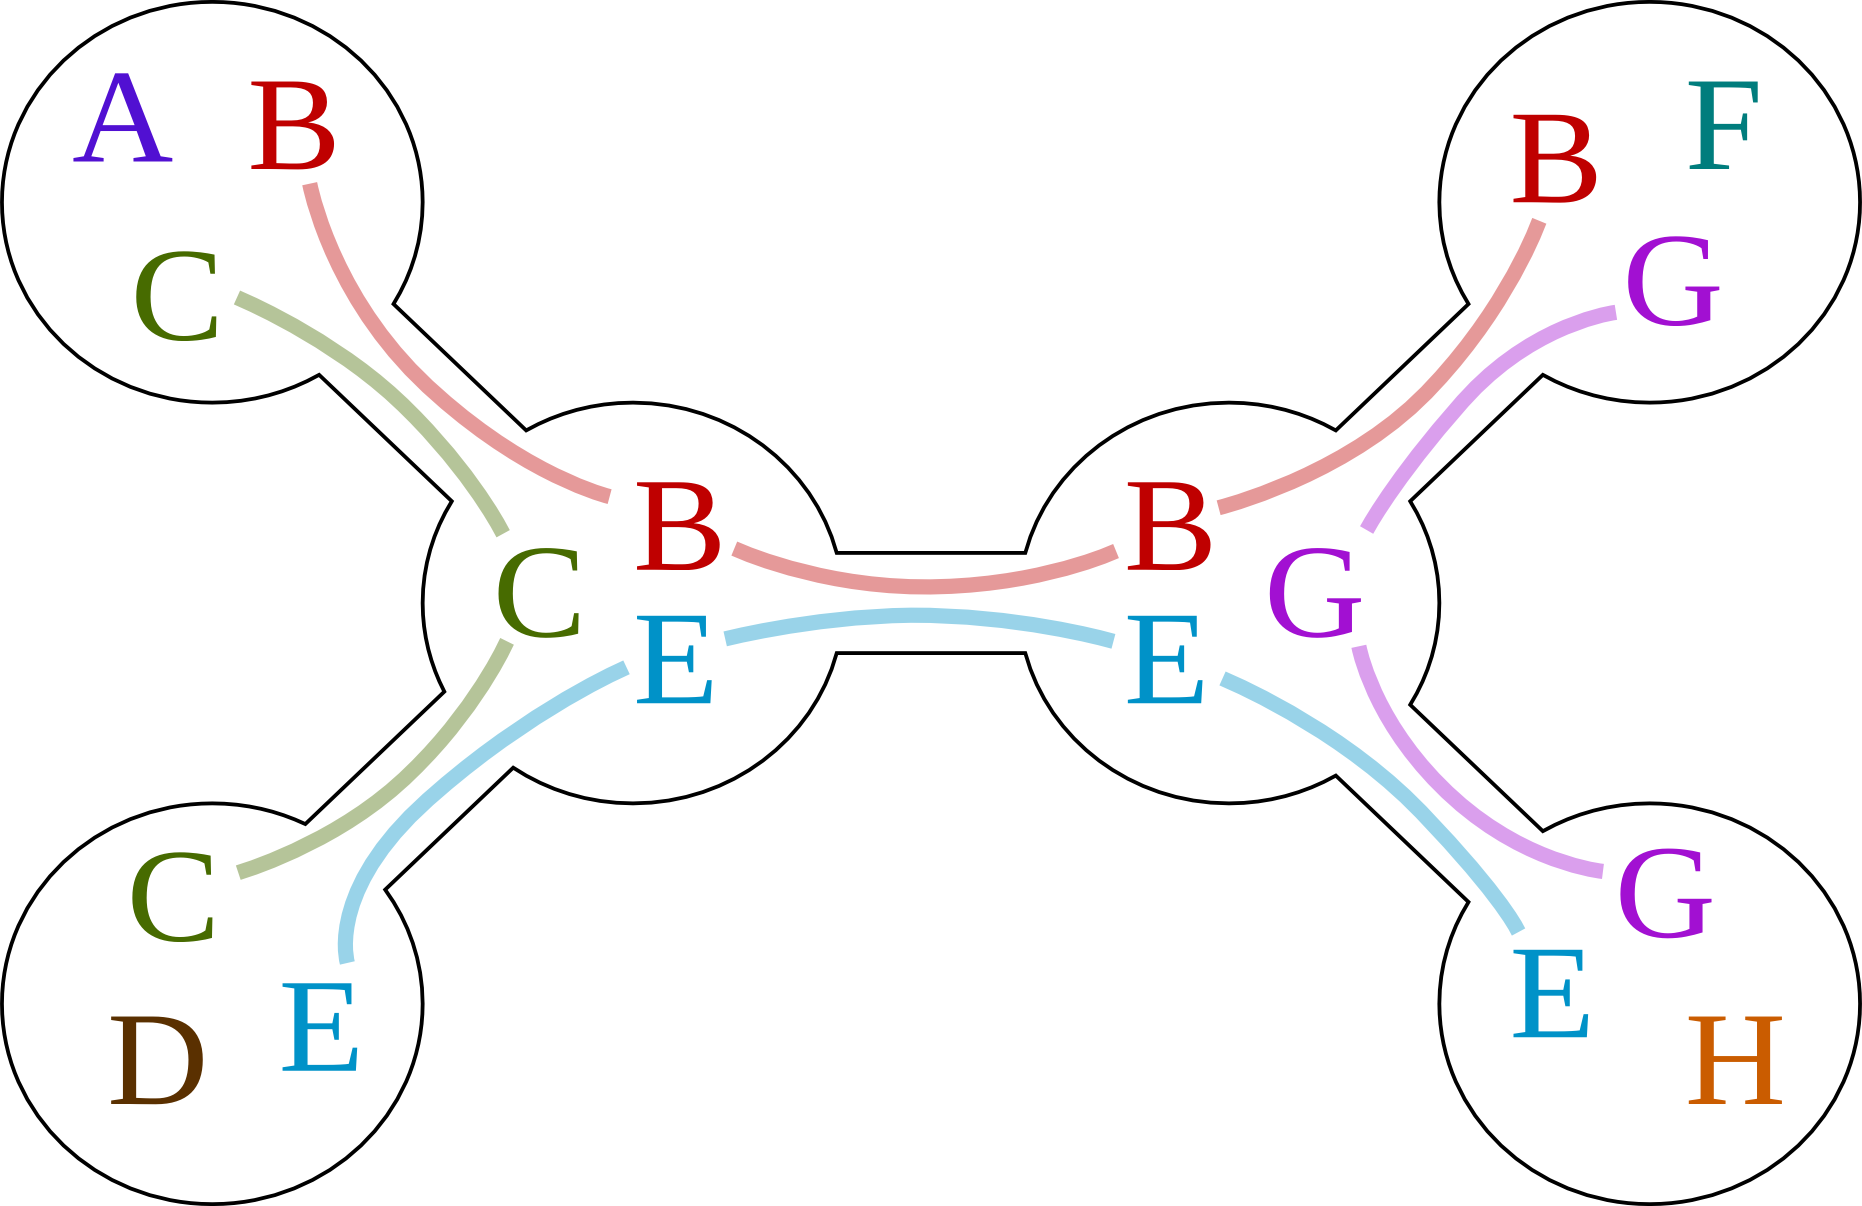
\includegraphics[height=0.37\textheight]{my_tree_4.png}
%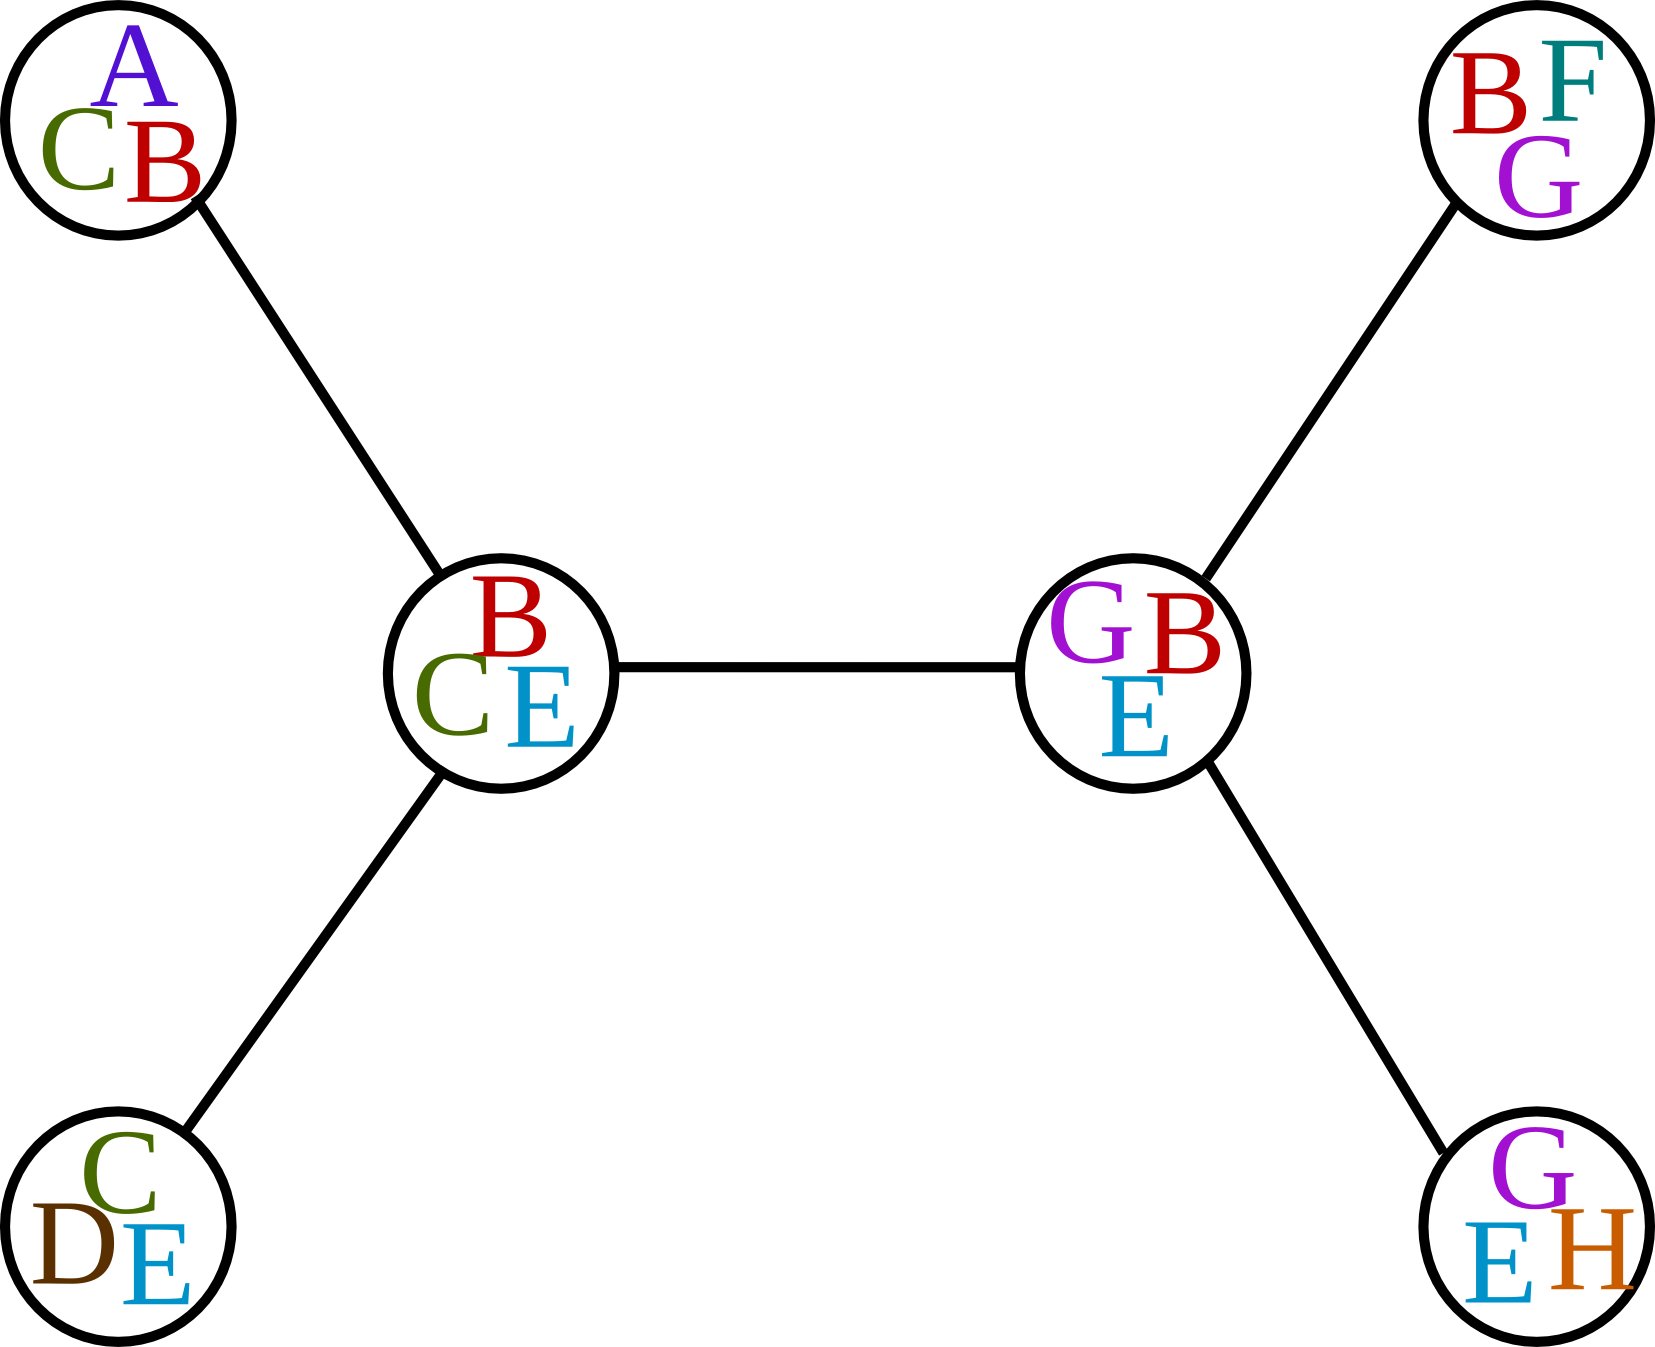
\includegraphics[height=0.3\textheight]{figures/my_tree_2.png} 
\end{center}

\begin{itemize}
\item definition and examples~\cite{krumke09}
\medskip
\item properties of tree decompositions (cliques, minors)~\cite{krumke09}
\medskip
\item calculating tree decompositions of (chordal) graphs~\cite{krumke09}
\end{itemize}

\end{frame}


%%%%%%%%%%%%%%%%%%%
%         11       %
%%%%%%%%%%%%%%%%%%%
\begin{frame}
\frametitle{Greedy Graph Algorithms / Matroids}
\begin{block}{}
  matroids are  structures that generalize the notion of linear independence in matrices. Find a maximum weight independent set in a matroid
  %Find a maximum weight independent set in a matroid and solve the problem with greedy algorithm
\end{block}
  \begin{center}
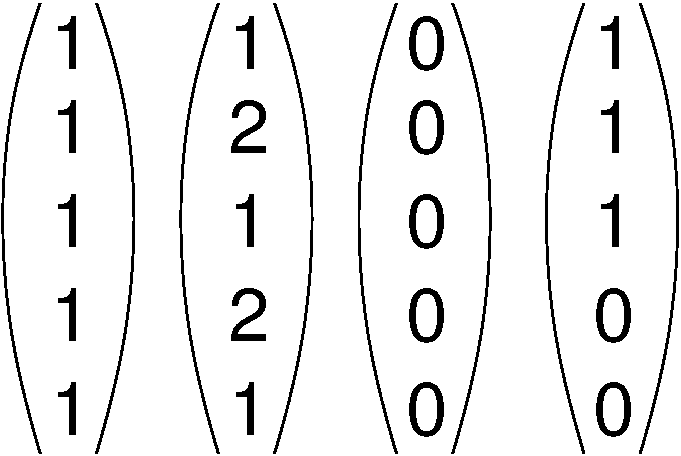
\includegraphics[height=0.2\textwidth]{vectors}\qquad \qquad
\includegraphics[height=0.25\textwidth]{mst}\qquad \qquad
\includegraphics[height=0.2\textwidth]{uniform}
\end{center}
~\\
\begin{itemize}
\item definition and examples of matroids~\cite{Oxley92,krumke09}
\item matroid optimization problem~\cite{Oxley92,krumke09}
\item greedy algorithm on matroids~\cite{Oxley92,krumke09}
\end{itemize}

\end{frame}

%%%%%%%%%%%%%%%%%%%
%         11       %
%%%%%%%%%%%%%%%%%%%
\begin{frame}
\frametitle{List of Topics}
\begin{enumerate}
\item Fast MST by Fredman and Tarjan
\item Approximation of Min-Steiner-Trees
\item The Edge Coloring Problem
\item The PageRank Algorithm
\item The Assignment Problem  
\item The Blossom Algorithm 
\item Minimum Cuts by Karger and Stein
\item Spectral Partitioning
\item Tree Decomposition
\item Greedy Graph Algorithms / Matroids

\end{enumerate}

\end{frame}


\begin{frame}[allowframebreaks]
        \frametitle{References}
        %        \bibliographystyle{amsalpha}
        \bibliographystyle{acm}
        \bibliography{biblio}
\end{frame}



%% %%%%%%%%%%%%%%%%%%%%%%%%%%%%%%%%%%%%%%%%%
%% %%%%%%%%%%%%%%%%%%%%%%%%%%%%%%%%%%%%%%%%%
%% \begin{frame}
%% \frametitle{References (1)}

%% \begin{itemize}
%% \item[1.]
%% R.~{Diestel}.\\
%% {\em {Graph Theory}}, volume 173 of {\em Graduate Texts in Mathematics}.\\
%% Springer, 2010.

%% \item[2.]
%% J.~{Edmonds}.\\
%% Paths, trees, and flowers.\\
%% {\em Canad. J. Math.}, 17:449--467, 1965.

%% \item[3.]
%% J.~{Eisner}.\\
%% State-of-the-art algorithms for minimum spanning trees - a tutorial discussion, 1997.

%% \end{itemize}
%% \end{frame}

%% %%%%%%%%%%%%%%%%%%%%%%%%%%%%%%%%%%%%%%%%%
%% \begin{frame}
%% \frametitle{References (2)}

%% \begin{itemize}
%% \item[4.]
%% A.~V. {Goldberg} and C.~{Harrelson}.\\
%% Computing the shortest path: $A^*$ search meets graph theory.\\
%% In {\em Proceedings of the Sixteenth Annual ACM-SIAM Symposium on
%%   Discrete Algorithms}, SODA '05, pages 156--165, Philadelphia, PA, USA, 2005.
%%   %Society for Industrial and Applied Mathematics.

%% \item[5.]
%% P.~E. {Hart}, N.~J. {Nilsson}, and B.~{Raphael}.\\
%% A formal basis for the heuristic determination of minimum cost paths.\\
%% {\em IEEE Transactions on Systems, Science, and Cybernetics},
%%   SSC-4(2):100--107, 1968.
%% \end{itemize}

%% \end{frame}

%% %%%%%%%%%%%%%%%%%%%%%%%%%%%%%%%%%%%%%%%%%
%% \begin{frame}
%% \frametitle{References (3)}

%% \begin{itemize}
%% \item[6.]
%% D.~R. {Karger} and C.~{Stein}.\\
%% A new approach to the minimum cut problem.
%% {\em J. ACM}, 43(4):601--640, 1996.

%% \item[7.]
%% S.O. Krumke and H.~Noltemeier.\\
%% {\em Graphentheoretische Konzepte und Algorithmen}.\\
%% Leitf{\"a}den der Informatik. Vieweg + Teubner, 2009.

%% \item[8.]
%% J.~{Misra} and D.~{Gries}.\\
%% A constructive proof of Vizing’s theorem.\\
%% {\em Information Processing Letters}, 41, 1992. 

%% \item[9.]
%% J.G. {Oxley}.\\
%% {\em Matroid theory}.\\
%% Oxford University Press, New York, USA, 1992.
%% \end{itemize}

%% \end{frame}

%% \begin{frame}
%% \frametitle{References (4)}

%% \begin{itemize}

%% \item[10.]
%% M.~Fiedler.\\
%% {\em Algebraic connectivity of Graphs}.\\
%%  Czechoslovak Mathematical Journal 23(98) (1973), 298?305.

%% \item[11.]
%% R.~Lipton, and R.~Tarjan.\\
%% {\em A separator theorem for planar graphs}.\\
%% Siam J. Appl. Math., Vol. 36, No. 2, pages 177?189, 1979.

%% \item[12.]
%% Micha Sharir.\\
%% \em{ A strong connectivity algorithm and its applications to data flow analysis}.\\
%% Computers and Mathematics with Applications 7(1):67?72, 1981.
%% \end{itemize}

%% \end{frame}

%% \begin{frame}
%% \frametitle{References (5)}

%% \begin{itemize}

%% \item[13.]
%% Tarjan,~R.~E.\\  
%% {\em Depth-first search and linear graph algorithms}.\\
%% SIAM Journal on Computing, 1 (2): 146?160, 1972.

%% \item[14.]
%% Bichot, Charles-Edmond and Siarry, Patrick.\\
%% {\em Graph Partitioning: Optimisation and Applications}.\\
%% John Wiley \& Sons, 24 Jan 2013.
%% \vfill\clearpage
%% \end{itemize}

%% \end{frame}



\end{document}
